%% 
%% Copyright 2019-2020 Elsevier Ltd
%% 
%% This file is part of the 'CAS Bundle'.
%% --------------------------------------
%% 
%% It may be distributed under the conditions of the LaTeX Project Public
%% License, either version 1.2 of this license or (at your option) any
%% later version.  The latest version of this license is in
%%    http://www.latex-project.org/lppl.txt
%% and version 1.2 or later is part of all distributions of LaTeX
%% version 1999/12/01 or later.
%% 
%% The list of all files belonging to the 'CAS Bundle' is
%% given in the file `manifest.txt'.
%% 
%% Template article for cas-dc documentclass for 
%% double column output.

%\documentclass[a4paper,fleqn,longmktitle]{cas-dc}
\documentclass[a4paper,fleqn]{cas-dc}

%\usepackage[authoryear,longnamesfirst]{natbib}
%\usepackage[authoryear]{natbib}
\usepackage[numbers]{natbib}

%%%Author definitions
\def\tsc#1{\csdef{#1}{\textsc{\lowercase{#1}}\xspace}}
\tsc{WGM}
\tsc{QE}
\tsc{EP}
\tsc{PMS}
\tsc{BEC}
\tsc{DE}
%%%

\begin{document}
\let\WriteBookmarks\relax
\def\floatpagepagefraction{1}
\def\textpagefraction{.001}
\shorttitle{Fingerprint reconstruction}
\shortauthors{Cristian Yesid Andrade et~al.}

\title [mode = title]{Fingerprint Reconstruction Using a Compact Convolutional Generative Adversarial Model}  


\cortext[1]{Corresponding author: Cristian Yesid Andrade, email: cy.andrade@uniandes.edu.co}
\author[1]{Cristian Yesid Andrade}\cormark[1]

\address[1]{Olimpia IT, Bogotá, Colombia}
\address[2]{Deptartment of Electric and Electronic Engineering, Universidad de los Andes, Cra 1 Nº 18A - 12, Bogotá, Colombia}


\author[2]{Luis Felipe Giraldo}
\author[1]{Daniel Medina}


% % AUTHOR 1
% \author{}
% \ead{cy.andrade@uniandes.edu.co}
% %\credit{Conceptualization of this study, Methodology, Software}

% % AUTHOR 2
% \author{Luis Felipe Giraldo}
% \ead{lf.giraldo404@uniandes.edu.co}
% %\credit{Thesis advisor}

% % AUTHOR 3
% \author{Daniel Medina}
% \ead{Daniel.Medina@olimpiait.com}


\begin{abstract}
%Biometric systems record fingerprints into digital platforms allowing governments and organizations to have a structured and reliable way to identify people. In some cases, uncontrolled factors in both enrollment and verification processes make the biometric systems to obtain poor quality fingerprints records. Thus, performance of automatic identification decreases and the work of dactyloscopists becomes harder. This paper describes the implementation of a convolutional generative adversarial model that performs fingerprint image reconstruction in order to obtain clear ridge patterns using TensorFlow. Fingerprint enhancement boosts the correct extraction of fingerprint features called minutiae which are the center of matching and identification algorithms. A biometric open source framework called NBIS is used to measure the efectiveness of the model in terms of matching accuracy and image quality.
Biometric systems that record and analyze fingerprints require high quality records to provide a reliable automatic identification. Poor quality records affect performance of the identification process. In this paper we describe the implementation of a convolutional generative adversarial model for fingerprint image reconstruction to obtain clear ridge patterns. We focus on situations where the fingerprint collection is conducted in controlled scenarios that are affected by factors such as acquisition device malfunctioning or skin deterioration. We evaluate the proposed model according to two criteria: i) matching accuracy and image quality using metrics proposed by the National Institute of Standards and Technology; and ii) computational load in real implementations when deployed on engines for real-time processing such as Raspberry Pi and a server through an API. We show the effectiveness of the model in terms of quality and practical implementation. 
%A biometric open source framework called NBIS is used to measure the efectiveness of the model in terms of matching accuracy and image quality.
\end{abstract}

\begin{keywords}
Fingerprint enhancement \sep generative adversarial  network \sep Deep Learning \sep Raspberry Pi
\end{keywords}

\maketitle
%%%%%%%%%%%%%%%%%%%%%%%%%%%%%%%%%%%%%%%%%%%%%%%%%%%%
\section{Introduction}
%Each minutia is determined by four values: pixel position in vertical axis, pixel position in horizontal axis, orientation and quality \cite{NBISUG}.
Fingerprint images are probably the most used  biometric marker for identity recognition \cite{HFPR}. Typically, algorithms for identity recognition analyze patterns in local ridge and valley characteristics of fingerprint images such as endings and bifurcations, known as minutia \cite{HFPR}. These algorithms compute a score based on comparing minutia of two fingerprint images, where two fingerprints are considered to belong to the same person if the score is above a given threshold. There are cases where quality of recorded fingerprints is poor, even in controlled situations, due to factors that include cuts, burnt skin, dryness, dermatitis, dirty scanning surfaces, and malfunction in acquisition devices \cite{HFPR,FIESDD,CCGAN,AIFEGF,OFFIE}. These factors either remove real minutia or create false ones, affecting the identification process. Hence, methods to reconstruct patterns in ridges and valleys in fingerprints are needed to improve the identification accuracy. During the last three decades, different methods for fingerprint enhancement and reconstruction have been proposed. Most of the restoration methods are based on local contextual analysis of the fingerprint, considering local ride orientation and local ridge frequency to estimate the correct pattern. Some of these methods analyze spatial  and frequency information to define a set of filters that conduct the reconstruction \cite{chikkerur2005fingerprint,fronthaler2007pyramid,turroni2012fingerprint,SIFE}. Other work add prior information on the patterns that are found in fingerprints to the reconstruction system to improve accuracy \cite{feng2010fingerprint,cao2014learning}   Most recent methods have focused on the use of deep convolutional neural networks to enhance fingerprints in a generative adversarial paradigm \cite{ITITAN,CCGAN,dabouei2018id,svoboda2017generative}. The resultant models are deep networks with a large amount of layers that are able to learn more sophisticated filters, allowing for the identification and analysis of fingerprint patterns. It has been shown that this scheme provides improved reconstruction results, providing that there are a large amount of fingerprint samples and computational resources for training. 
% %Diferencias:
% - Enfoque de otros que trabajan con GANs en latent fingerprints
% - Mas compacto para implementacions portables
% - Utilizacion de U-net: aprovechan informacion de alto nivel y bajo nivel en modelo de reconstruccion, dan contexto a la reconstruccion, ayuda la red a ser mas compacta. 

Even though a great deal of research has been conducted to analyze fingerprint images, fingerprint reconstruction in biometric systems is still an open problem. In this paper, we focus on the scenario where the fingerprint image is collected using acquisition devices in controlled situations such as a bank, police check, military operations, and biometric entrance guard control. The main challenge in this scenario for fingerprint image reconstruction lies in the development of a model that is accurate, portable, and provides low reconstruction times. Most of the recent work that has studied deep neural networks for fingerprint enchancement and reconstruction has focused on reconstructing latent fingerprints and has developed very accurate models at the expense of having a large amount of layers that increase computational processing times. Our contribution in this document is to propose a model based on deep convolutional neural networks that is able i) to accurately reconstruct fingerprints in controlled scenarios, and ii) to provide fast processing times in portable devices for local reconstruction. We treat fingerprint enhancement as an image-to-image translation problem in a generative adversarial network framework \cite{ITITAN,goodfellow2016deep}, which we hypothesize can provide a compact reconstruction model through the analysis of high and low level information of the fingerprints (Section \ref{sec:PM}). To train and test our model, we used a database with 20.000 anonymous fingerprint images that were artificially modified to simulate two different types of deterioration that are commonly seen in controlled scenarios (Section \ref{sec:ER}). We used a metric proposed by the National Institute of Standards and Technology to measure the quality of the deteriorated, enhanced, and original images. Also, we deployed the model to a Raspberry Pi and evaluated the computational load required by our model to provide a local reconstruction of fingerprints (Section \ref{sec:CLT}). We ended this paper with a conclusion and future research directions (Section \ref{sec:FW}). 


%It consists of a set of interconnected layers that receive an image as input, processes it with convolutions and returns the expected image as output. Parameters of the layer's filters are modified through an optimization process that minimize a cost function using a similarity measure and the adversarial training paradigm.
%The paper follows the next organization: source and preprocessing of training data are described in section \hyperref[sec:DP]{2.1}. Section \hyperref[sec:MA]{2.2} presents model architecture details. Training configuration is explained in section \hyperref[sec:MT]{2.3}. Section \hyperref[sec:R]{3} presents and analyses results. Then, section \hyperref[sec:CLT]{4} describes a compute load test. Finally, conclusion and future work are in sections \hyperref[sec:FW]{5} and \hyperref[sec:FW]{6} respectively.
     
     
     
%%%%%%%%%%%%%%%%%%%%%%%%%%%%%%%%%%%%%%%%%%%%%%%     
\section{Proposed Methodology}
\label{sec:PM}

%%%%%%%%%%%%%%%%%%%%%%%%%%%%%%%%%%%%%%%%%%%%%%%%
\subsection{Data Collection and Preprocessing}
\label{sec:DP}
We collected a dataset with 100.000 fingerprint images that were recorded during the driver's licence examination in Colombia, South America. Each sample corresponded to a 256x256 pixel image recorded using the optical device Morpho smart MSO 1300 V3. Figure \ref{fig1} shows some examples of the fingerprint images in the dataset.
\begin{figure}[ht]
\centerline{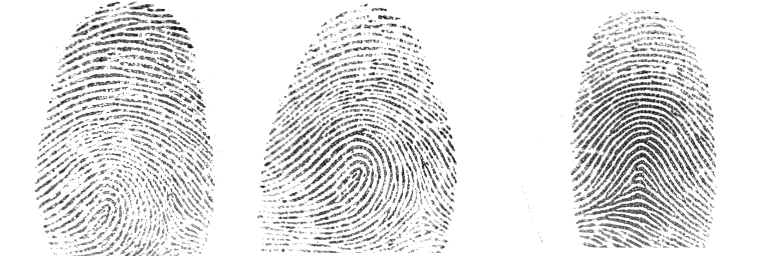
\includegraphics[scale=0.3]{figs/dataset_example.png}}
\caption{Example images from the collected dataset.}
\label{fig1}
\end{figure}
To train and test the fingerprint image reconstruction system, we built tuples of images, each with an image to enhance and a target image. The image to enhance is obtained through an artificial deterioration process and the target image is the original image of the dataset. There are two types of deterioration that are commonly seen in controlled fingerprint acquisition scenarios. The first type of fingerprint deterioration is obtained by overlapping random white ellipses on the fingerprint and adding a Gaussian noise to simulate a skin disease, a burnt finger, or other types of fingerprint modifications. Figure \ref{fig2} shows an example of this type of image deterioration.
\begin{figure}[htbp]
\centerline{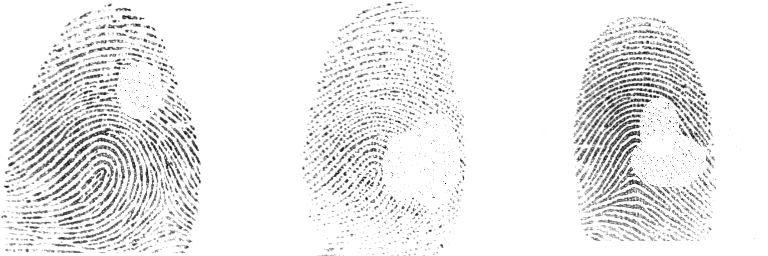
\includegraphics[scale=0.3]{figs/deterioration_1.png}}
\caption{Artificial fingerprint deterioration with holes}
\label{fig2}
\end{figure}
The second type of deterioration tries to simulate wet/dry fingers and dirty scanning surfaces. This is obtained by adding a fixed value to every pixel in the image until the mean of the image reaches 250 to remove some ridges and to blur the image. Also, a Gaussian noise is added as shown in Fig.~\ref{fig3}.
\begin{figure}[ht]
\centerline{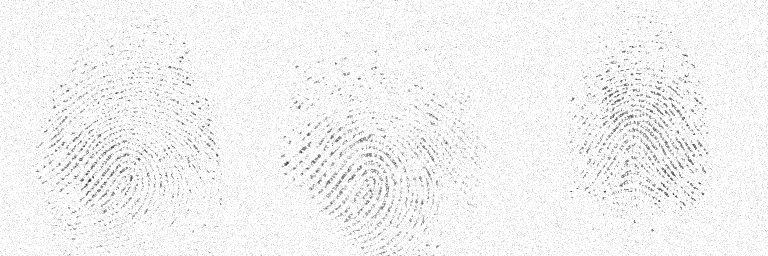
\includegraphics[scale=0.32]{figs/deterioration_2.png}}
\caption{Artificial fingerprint deterioration simulating finger or scanning modified conditions}
\label{fig3}
\end{figure}


%%%%%%%%%%%%%%%%%%%%%%%%%%%%%%%%%%%%%%%%%%%%%%%%%%%%
\subsection{Model Architecture}\label{sec:MA}
The proposed architecture is composed of a generator that receives the image to enhance as input and returns the reconstructed image as output and a discriminator that determines whether or not an image was successfully reconstructed. \textcolor{green}{Figure \ref{fig:diagramGenDis} shows a flow diagram that describes how the generator and discriminator cost functions are calculated in order to perform an iterative parameters update.}\textcolor{red}{en esta explicacion, hablar un poco del diagrama de bloques de la figura 4. Falta hablar, por ejemplo, de la funcion de costo. Aqui se podria hablar sin mucho detalle. Algo muuuy general, que prepare el lector para los detalles que vienen despues.}.



\begin{figure}[!ht]
\centerline{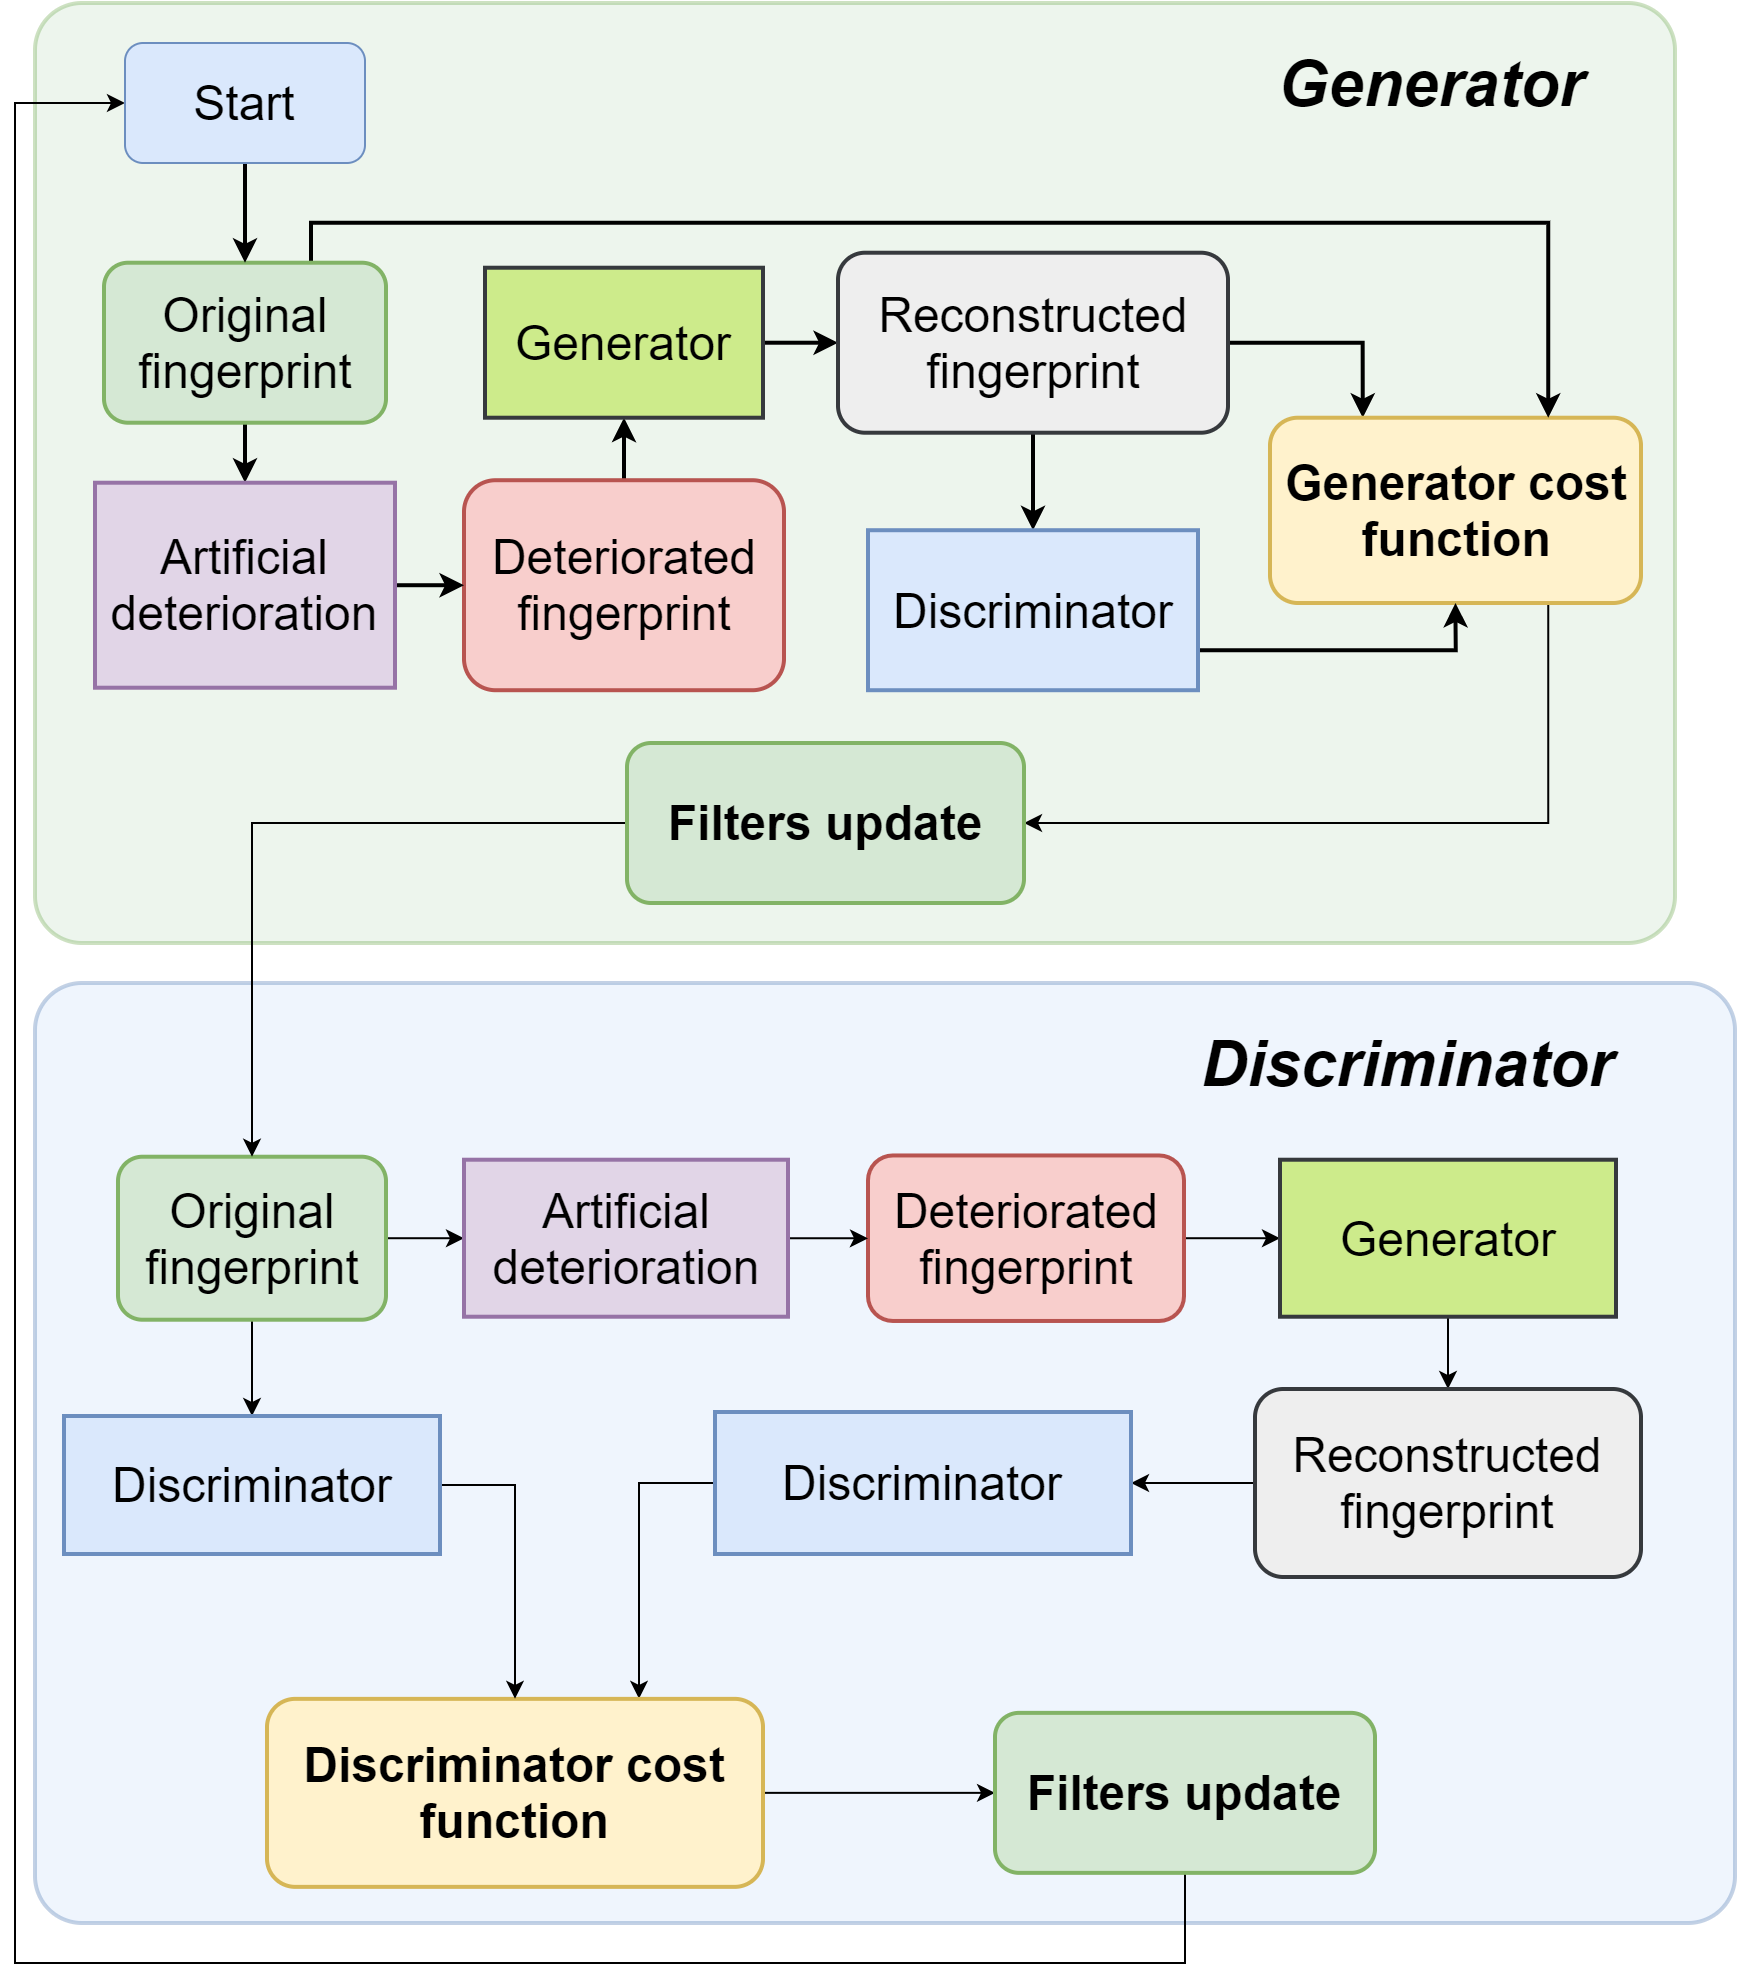
\includegraphics[scale=0.4]{figs/training_fd_en_v.png}}
\caption{Training flow}
\label{fig:diagramGenDis}
\end{figure}
The generator block contains an encoder and a decoder that configure an U-Net structure \cite{UNBIS}. The encoder is constructed using eight sequentially connected convolutional layers, each one reducing the input height and width by a factor of two using same padding and strides of two. All layers use leakyrelu activation and batch normalization, except for the first one. Similarly, the decoder is constructed using eight transposed convolutional layers, sometimes mistakenly called deconvolutional layers \textcolor{green}{\cite{dumoulin2016guide}} \textcolor{red}{citar literatura de esto de 'mistakenly'}. Here, decoder layers increment by a factor of two height and width of input volumes which results in a final image of 256x256 pixels. All layers use batch normalization and relu activation and the first three layers use drop regularization. Fig.~\ref{fig4} shows a sketch of the generator and Table~\ref{tab1} of appendix specifies architecture details including number of filters on each layer.
\begin{figure}[htbp]
\centerline{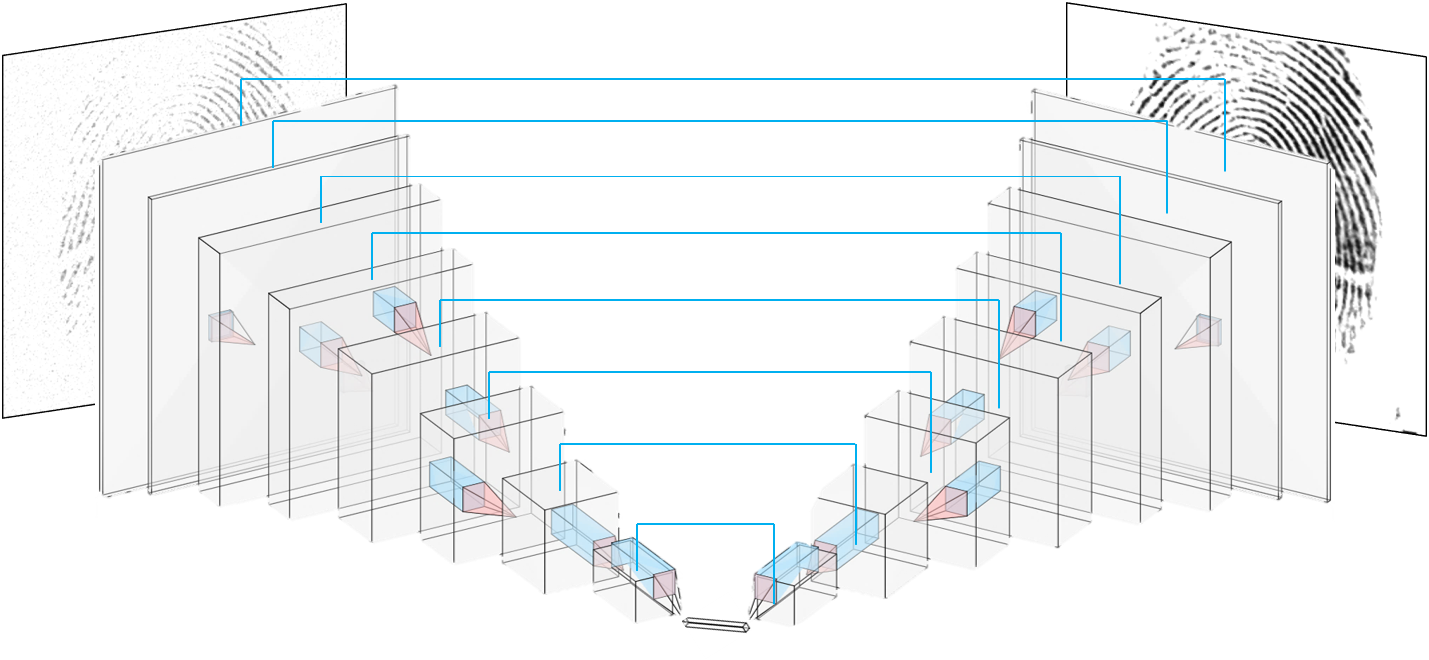
\includegraphics[scale=0.36]{figs/generador_p.png}}
\caption{Generator architecture}
\label{fig4}
\end{figure}
The discriminator block has a similar function to an encoder block since it applies convolutions to extract features from the input. \textcolor{green}{However, unlike standard GANs, discriminator output corresponds to a 29x29 volume where each value in interpreted as a projection of a 70x70 region of the input image. A sigmoid function is applied to each value of the volume and results are weighted to obtain the final scalar that represents the discriminator decision.} Fig.~\ref{fig5} shows a sketch of the discriminator and Table~\ref{tab2} of appendix specifies architecture details including number of filters on each layer. \textcolor{red}{Esta enredado este parrafo.}
\begin{figure}[htbp]
\centerline{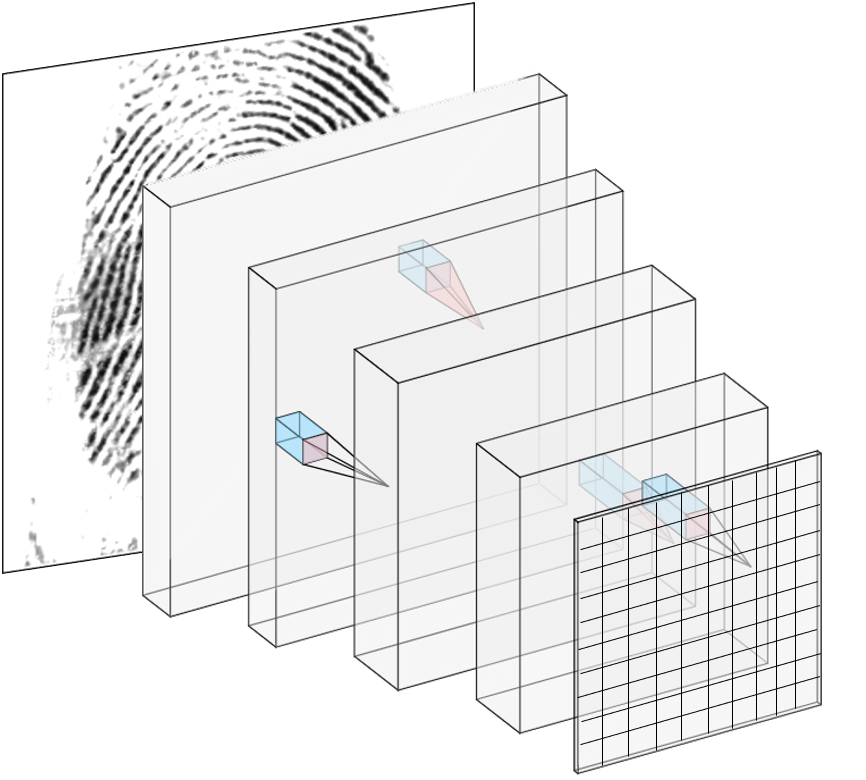
\includegraphics[scale=0.36]{figs/discriminador_p.png}}
\caption{Discriminator architecture}
\label{fig5}
\end{figure}

%%%%%%%%%%%%%%%%%%%%%%%%%%%%%%%%%%%%%%%%%%%%%%%%%%%%%
\subsection{Model Training}
\label{sec:MT}
The main objective of the reconstruction model is to make the generator reconstruct and enhance deteriorated fingerprints. To achieve that, the model is trained through an optimization process that finds the parameters of the deep networks in both the generator and the discriminator blocks. Since it is an adversarial architecture, there are two cost functions that drive the optimization. The first cost function is associated to the generator and contains the sum of two terms. To compute the first term, a deteriorated fingerprint of the dataset is passed through the generator. The reconstructed image is then compared to its ground truth using the L1 norm. The second term is computed by concatenating reconstructed and deteriorated image, and then passing the concatenation through the discriminator. \textcolor{green}{Finally cross-entropy is calculated using discriminator output as the estimated probability and 1 as the real probability. The fact of defining the real probability as 1 means the intent of generator to fool the discriminator.} \textcolor{red}{no se entiende esto del label. Nunca lo había mencionado antes} The concatenation of the deteriorated image gives to the discriminator a context that helps to improve optimization process. The following expression corresponds to the cost function:
\begin{equation}
    Gen_{loss} = \alpha||y-gen(x)||_{[1]} - \log(disc(x,gen(x)))
\end{equation}
Here, $x$ corresponds to the deteriorated image, $gen(x)$ is the reconstructed image, $y$ is the ground truth image, and $disc(x,gen(x))$ is the probability \textcolor{green}{that the fingerprint reconstruction has resulted successfully} \textcolor{red}{Probabilidad de que???}. Parameter $\alpha$ defines the weight of the reconstruction term in the optimization process.


The second cost function is the one that drives the learning process in the discriminator block. It also contains the sum of two terms: the first term is obtained by concatenating reconstructed and deteriorated image, then passing the result through the discriminator. \textcolor{green}{Cross-entropy is calculated using discriminator output as the estimated probability and 0 as the real probability. Real probability is changed to 0 in order to express the intent of discriminator of not being fooled by the generator} \textcolor{red}{igual aqui hay que explicar bien esta parte. No se habia explicado antes lo del label, y lo de engañar al discriminador}. \textcolor{green}{The second term is calculated similarly, however, it is used the ground truth fingerprint instead of the reconstructed one. In this case real probability of cross entropy is equal to 1 which indicates that ground truth image is a correct reconstructed fingerprint} \textcolor{red}{estas ultimas lineas no se entienden.} The expression of this cost function is given by
\begin{equation}
    Disc_{loss} = -\log(1-disc(x,gen(x)))-\log(disc(x,y)).
\end{equation}
The training process is configured as follows: tuples formed in the preprocessing step are grouped into batches of 48 elements. \textcolor{green}{We used the ADAM optimizer, which computes first order gradient of stochastic objective functions, based on adaptive estimates of lower order \cite{kingma2014adam}. \textcolor{red}{XXXXXX...citar referencia del adam optimizaer}.} Parameters of the algorithm are set to $\beta_{1}=0.5$, $\beta_{2}=0.999$, a learning rate of $0.00018$ and \textcolor{green}{112 epochs}. To favor a correct reconstruction, $\alpha$ is set to 40. \textcolor{red}{Numero de iteraciones, hay mas detalles del entrenamiento del modelo que se pueden colocar?}


%%%%%%%%%%%%%%%%%%%%%%%%%%%%%%%%%%%%%%%%%%%%%%%%%%%
\section{Experimental Results}\label{sec:ER}
Two main software frameworks were used to develop and evaluate the reconstruction model: Tensorflow open source platform for building and training the model, and NIST Biometric Image Software (NBIS), an open source biometric framework with core capabilities on fingerprint image processing developed by the National Institute of Standards and Technology (NIST) for the Federal Bureau of Investigation (FBI) and Department of Homeland Security (DHS) \cite{NBISWP}. We used Tensorflow framework in Python programming language, taking advantage of GPU processing power of the Nvidia Tesla K40 graphic card.

Three NBIS modules were used in the project. \textcolor{green}{\textit{mindtct} module takes a fingerprint image and extracts location, orientation, type, and quality of each minutiae in the image. To do so, the algorithm generates quality, direction, contrast and curve maps which are used to binarize the image and extract minutiae. False minutiae is removed in the last step.} \textcolor{red}{Hablar un poco mas de este modulo}. \textcolor{green}{\textit{bozorth3} module computes a similarity score between either a pair or a list of pairs of minutiae. This is achieved by first constructing intra fingerprint minutia comparison tables, then constructing an inter fingerprint compatibility table and finally traversing the inter fingerprint compatibility table.} \textcolor{red}{Hablar un poco mas de este modulo y el algoritmo.} \textcolor{green}{\textit{nfiq} module uses a multi layer perceptron neural network classifier to compute a quality measure of fingerprints. Neural network input corresponds to a feature vector of quality image “map” and minutiae quality statistics obtained through mindtct module.} \textcolor{red}{Hablar un poco mas de este modulo} \cite{UGNBIS}.


Fig.~\ref{fig6} shows three enhanced fingerprints using the proposed method and the first type of deterioration. It can be seen that the model was able to reconstruct the corrupted regions drawing the ridges that had been disappeared.
\begin{figure}[!ht]
\centerline{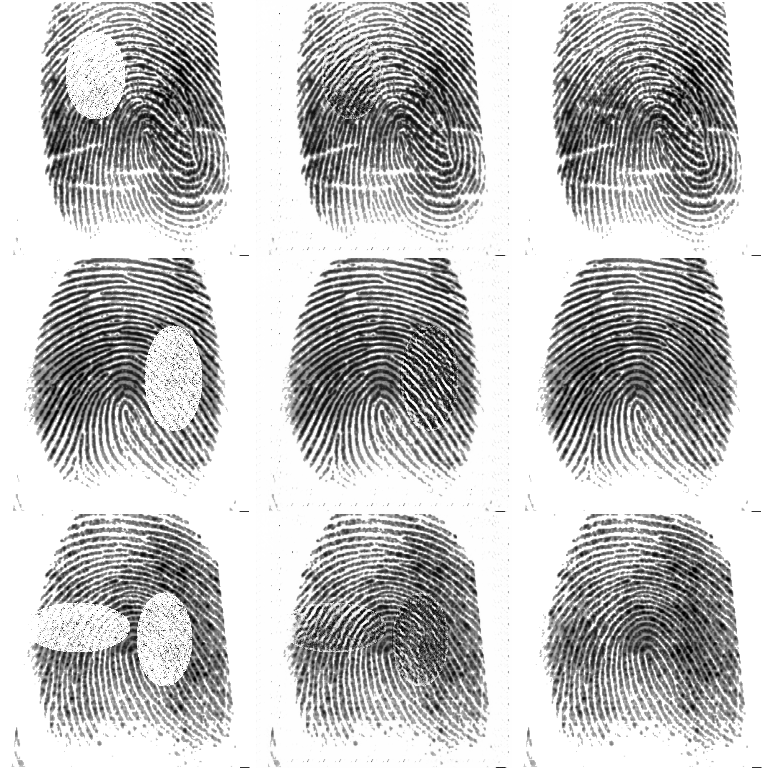
\includegraphics[scale=0.28]{figs/recons_1.png}}
\caption{Three examples of successful image reconstruction. First column has deteriorated images, the second column has the enhanced fingerprint images, and the third column has the ground truth images.}
\label{fig6}
\end{figure}
The reconstruction of fingerprints with the second type of deterioration is shown in Fig.~\ref{fig7}. Note that most of the ridges were recovered and the noise was diminished, improving fingerprint clarity and quality.
\begin{figure}[!ht]
\centerline{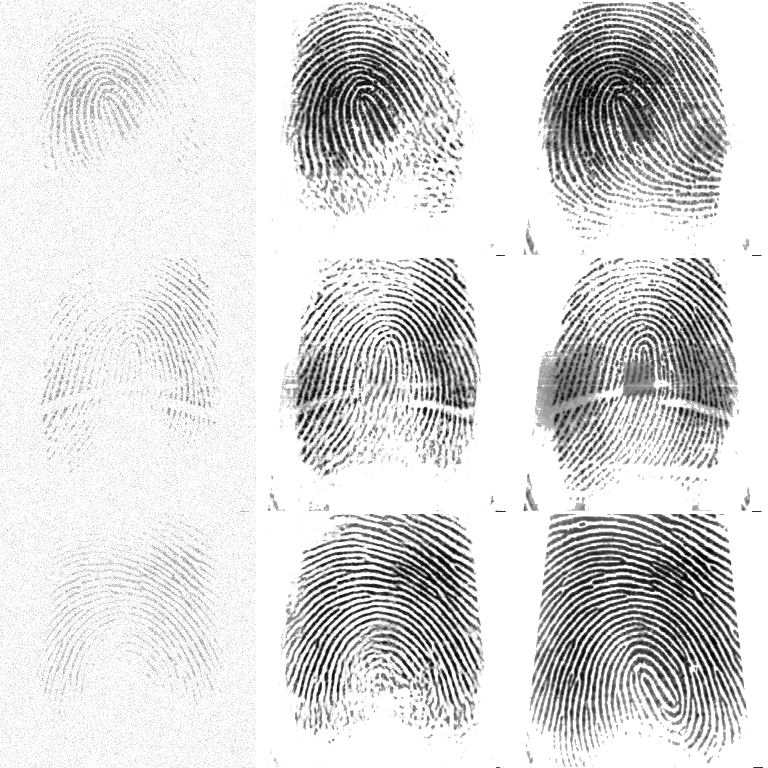
\includegraphics[scale=0.28]{figs/recons_2.png}}
\caption{Three examples of successful enhancement. First column has the deteriorated images, the second column has the enhanced fingerprint images, and the third column has the ground truth images.}
\label{fig7}
\end{figure}
On the other hand, Fig.~\ref{fig8} shows some fingerprint examples that could not be restored accurately. In these cases, the deterioration caused a high level of corruption in the fingerprints, making it almost impossible to achieve a successful enhancement. It is important to mention that if the fingerprints are highly corrupted or deteriorated, the model will not be not able to make a successful reconstruction. This is because the learned filters in the neural networks used to compute convolutions need a minimum information to extract features and represent them correctly in the output image.

% Also, fingerprints itself had noisy structures and saturated ridges that got over the algorithm capacity.
\begin{figure}[htbp]
\centerline{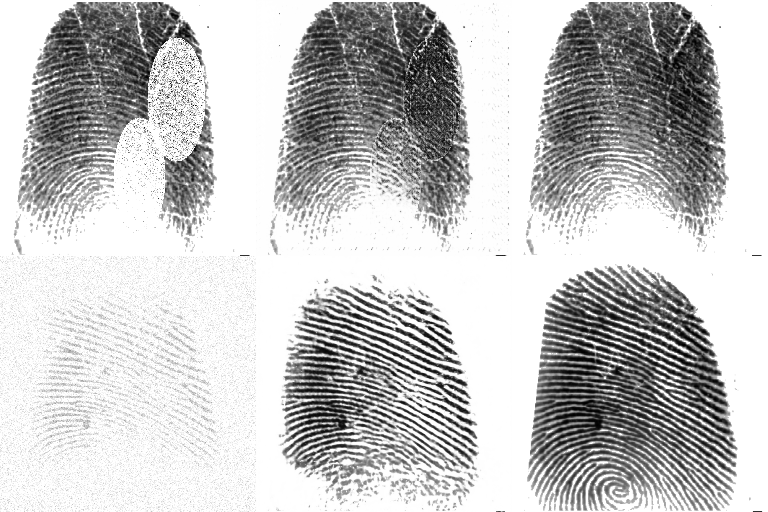
\includegraphics[scale=0.28]{figs/recons_failed.png}}
\caption{Two failed examples. First column is the deteriorated image, the second column is the enhanced fingerprint and the third column is the ground truth}
\label{fig8}
\end{figure}

\subsection{Matching and Quality Test}
\textcolor{red}{Como dividio el conjunto de datos para entrenamiento y test???} \textcolor{green}{90\% of the fingerprint dataset was used for training and 10\% for validation.} We conducted a first test to evaluate the model's performance using a 1:1 matching score computed \textcolor{green}{ using bozorth3 module.} \textcolor{red}{como se calcula el matching score? Con el software del NIST?}. Having two images, we say that these two images match if the matching score is above a given threshold. From the test set, we calculated the Receiver Operating Characteristic (ROC), a well-accepted measure to express performance of one-to-one matchers \cite{RROCCMC}. This curve is plotted by computing the True Positive Rate (TPR) and False Positive Rate (FPR) for different thresholds as can be seen in Fig.~\ref{fig9}. We compared two different ROC curves: one computed between images to reconstruct and the ground truth images, and another one computed between reconstructed images and ground truth images. 
\begin{figure}[!ht]
\centerline{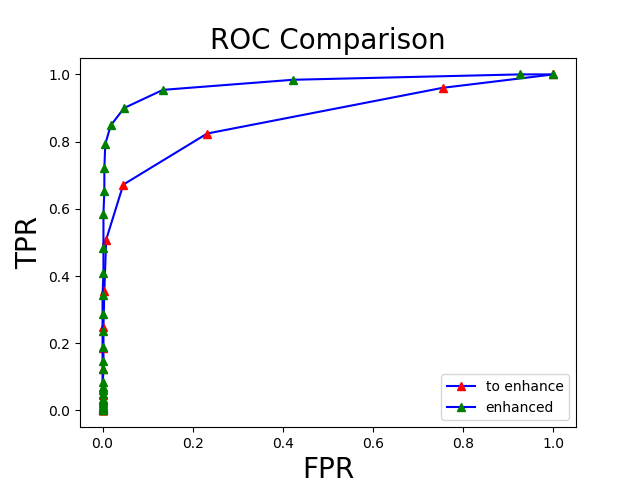
\includegraphics[scale=0.5]{figs/roc_comparison.png}}
\caption{ROC curve comparison before and after reconstruction}
\label{fig9}
\end{figure}
Since TPR stays at vertical axis and FPR at horizontal axis, a curve that is skewed to the left indicates better the model performances. Note that after reconstruction, true positive rate improved, meaning that the number of times that the model accepted a correct person increased. Also, false positive rate decreased,  meaning that the number of times that the model accepted a incorrect person decreased. Additionally, the area under the curve increased from 0.85 to 0.92, implying that the model for fingerprint recognition improved the accuracy of the matching process.

\textcolor{green}{We also conducted a second test where the CMC curve was computed to measure a 1:m biometric validation performance. \cite{RROCCMC}. CMC curve shows the cumulative probability of obtaining a correct match based on scores calculated between every possible tuple of fingerprint images.} Figure \ref{fig10} shows the results of computing two CMCs: one between tuples of deteriorated images and a ground truth images, and another one between enhanced images and ground truth images. Note that the enhanced fingerprints curve presents a higher value at $k$ equal to one and a steeper slope at that point. This indicates a better performance while implementing a 1:m fingerprint identification algorithm through sorting \cite{RROCCMC}. \textcolor{red}{Todo este parrafo esta enredado (desde donde dice 'we also conducted').}
\begin{figure}[htbp]
\centerline{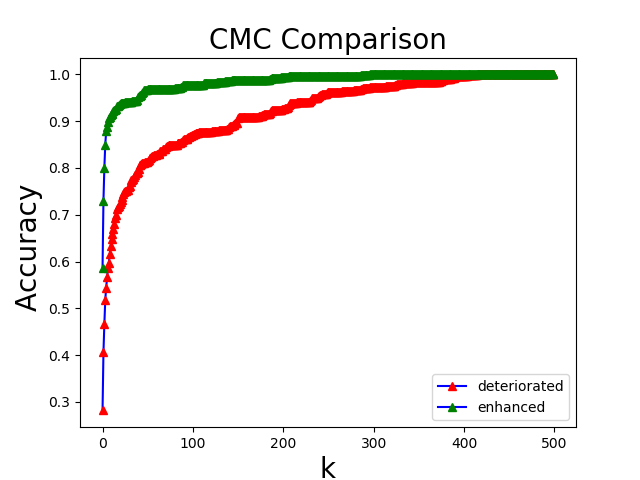
\includegraphics[scale=0.5]{figs/cmc_comparison.png}}
\caption{CMC curve comparison before and after reconstruction}
\label{fig10}
\end{figure}

The final performance metric quantifies the average fingerprint image quality of the validation dataset before and after reconstruction. \textcolor{green}{NFIQ fingerprint image quality is defined as a predictor of a matcher’s performance \cite{Tabassi2009}.} \textcolor{red}{Aqui en este contexto que significa quality???}. We used the nfiq module of the NBIS to do this. This module assigns a value of 1 to a fingerprint with the highest quality, and a value of 5 to the lowest quality fingerprint. That is, lower values of this measure indicate higher quality fingerprints.  Fig.~\ref{fig11} shows the results. Here, note that after enhancement, fingerprints deterioration level decreased from an average score of 3.9 to 2.72, that is, approximately a reduction of 43\%.
\begin{figure}[htbp]
\centerline{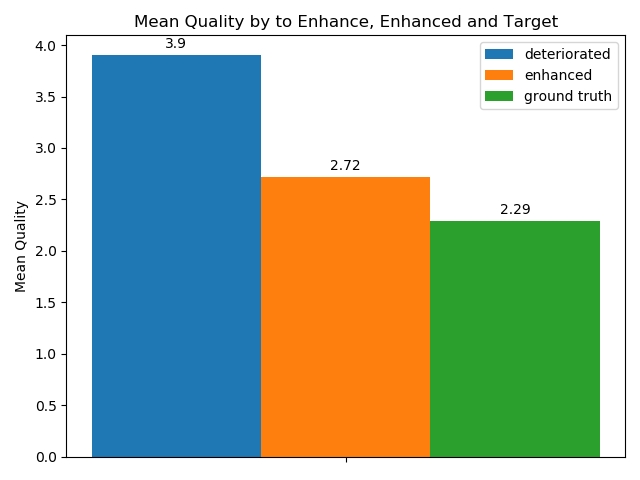
\includegraphics[scale=0.54]{figs/mean_qualities.png}}
\caption{Deterioration level comparison before and after reconstruction. \textcolor{red}{Quitar la palabra qualities del eje horizontal. Ya tiene un legend que es informativo.} \textcolor{green}{Listo}}
\label{fig11}
\end{figure}

%%%%%%%%%%%%%%%%%%%%%%%%%%%%%%%%%%%%%%%%%%%%%%%%%%
\subsection{Computational Load Test}
\label{sec:CLT}
To measure computational feasibility for implementation of the model, 300 fingerprints were reconstructed using two different engines. First, we used a Raspberry PI, a practical device where light and portable tech solutions can be implemented. The second engine corresponds to a simulation of a server running a fingerprint reconstruction API. Table \ref{table:computational_load} shows the average computational load in these two scenarios. These results show that the model can be easily implemented in both a lightweight portable device and a standard web server, providing reconstruction times per fingerprint low enough to build real-time image processing applications, and enabling us to deploy a commercial solution.
\begin{table}[h!]\label{table:computational_load}
\caption{Average computational load for 300 fingerprint images reconstruction.}
\centering
 \begin{tabular}{|lll|} 
 \hline
 Device & Process & Computational load\\ 
 \hline
 Raspberry Pi & RAM & 593 MB \\ 
 Raspberry Pi & Reconstruction time & 1.4s \\
 Server & RAM & 612 MB \\ 
 Server & Reconstruction time & 0.2s \\ 
 \hline
 \end{tabular}
\end{table}

% %During enhancement process, RAM memory consumed by the device was in average 593 MB and mean reconstruction time per fingerprint was 1.4 seconds.
% \begin{figure}[!ht]
% \centerline{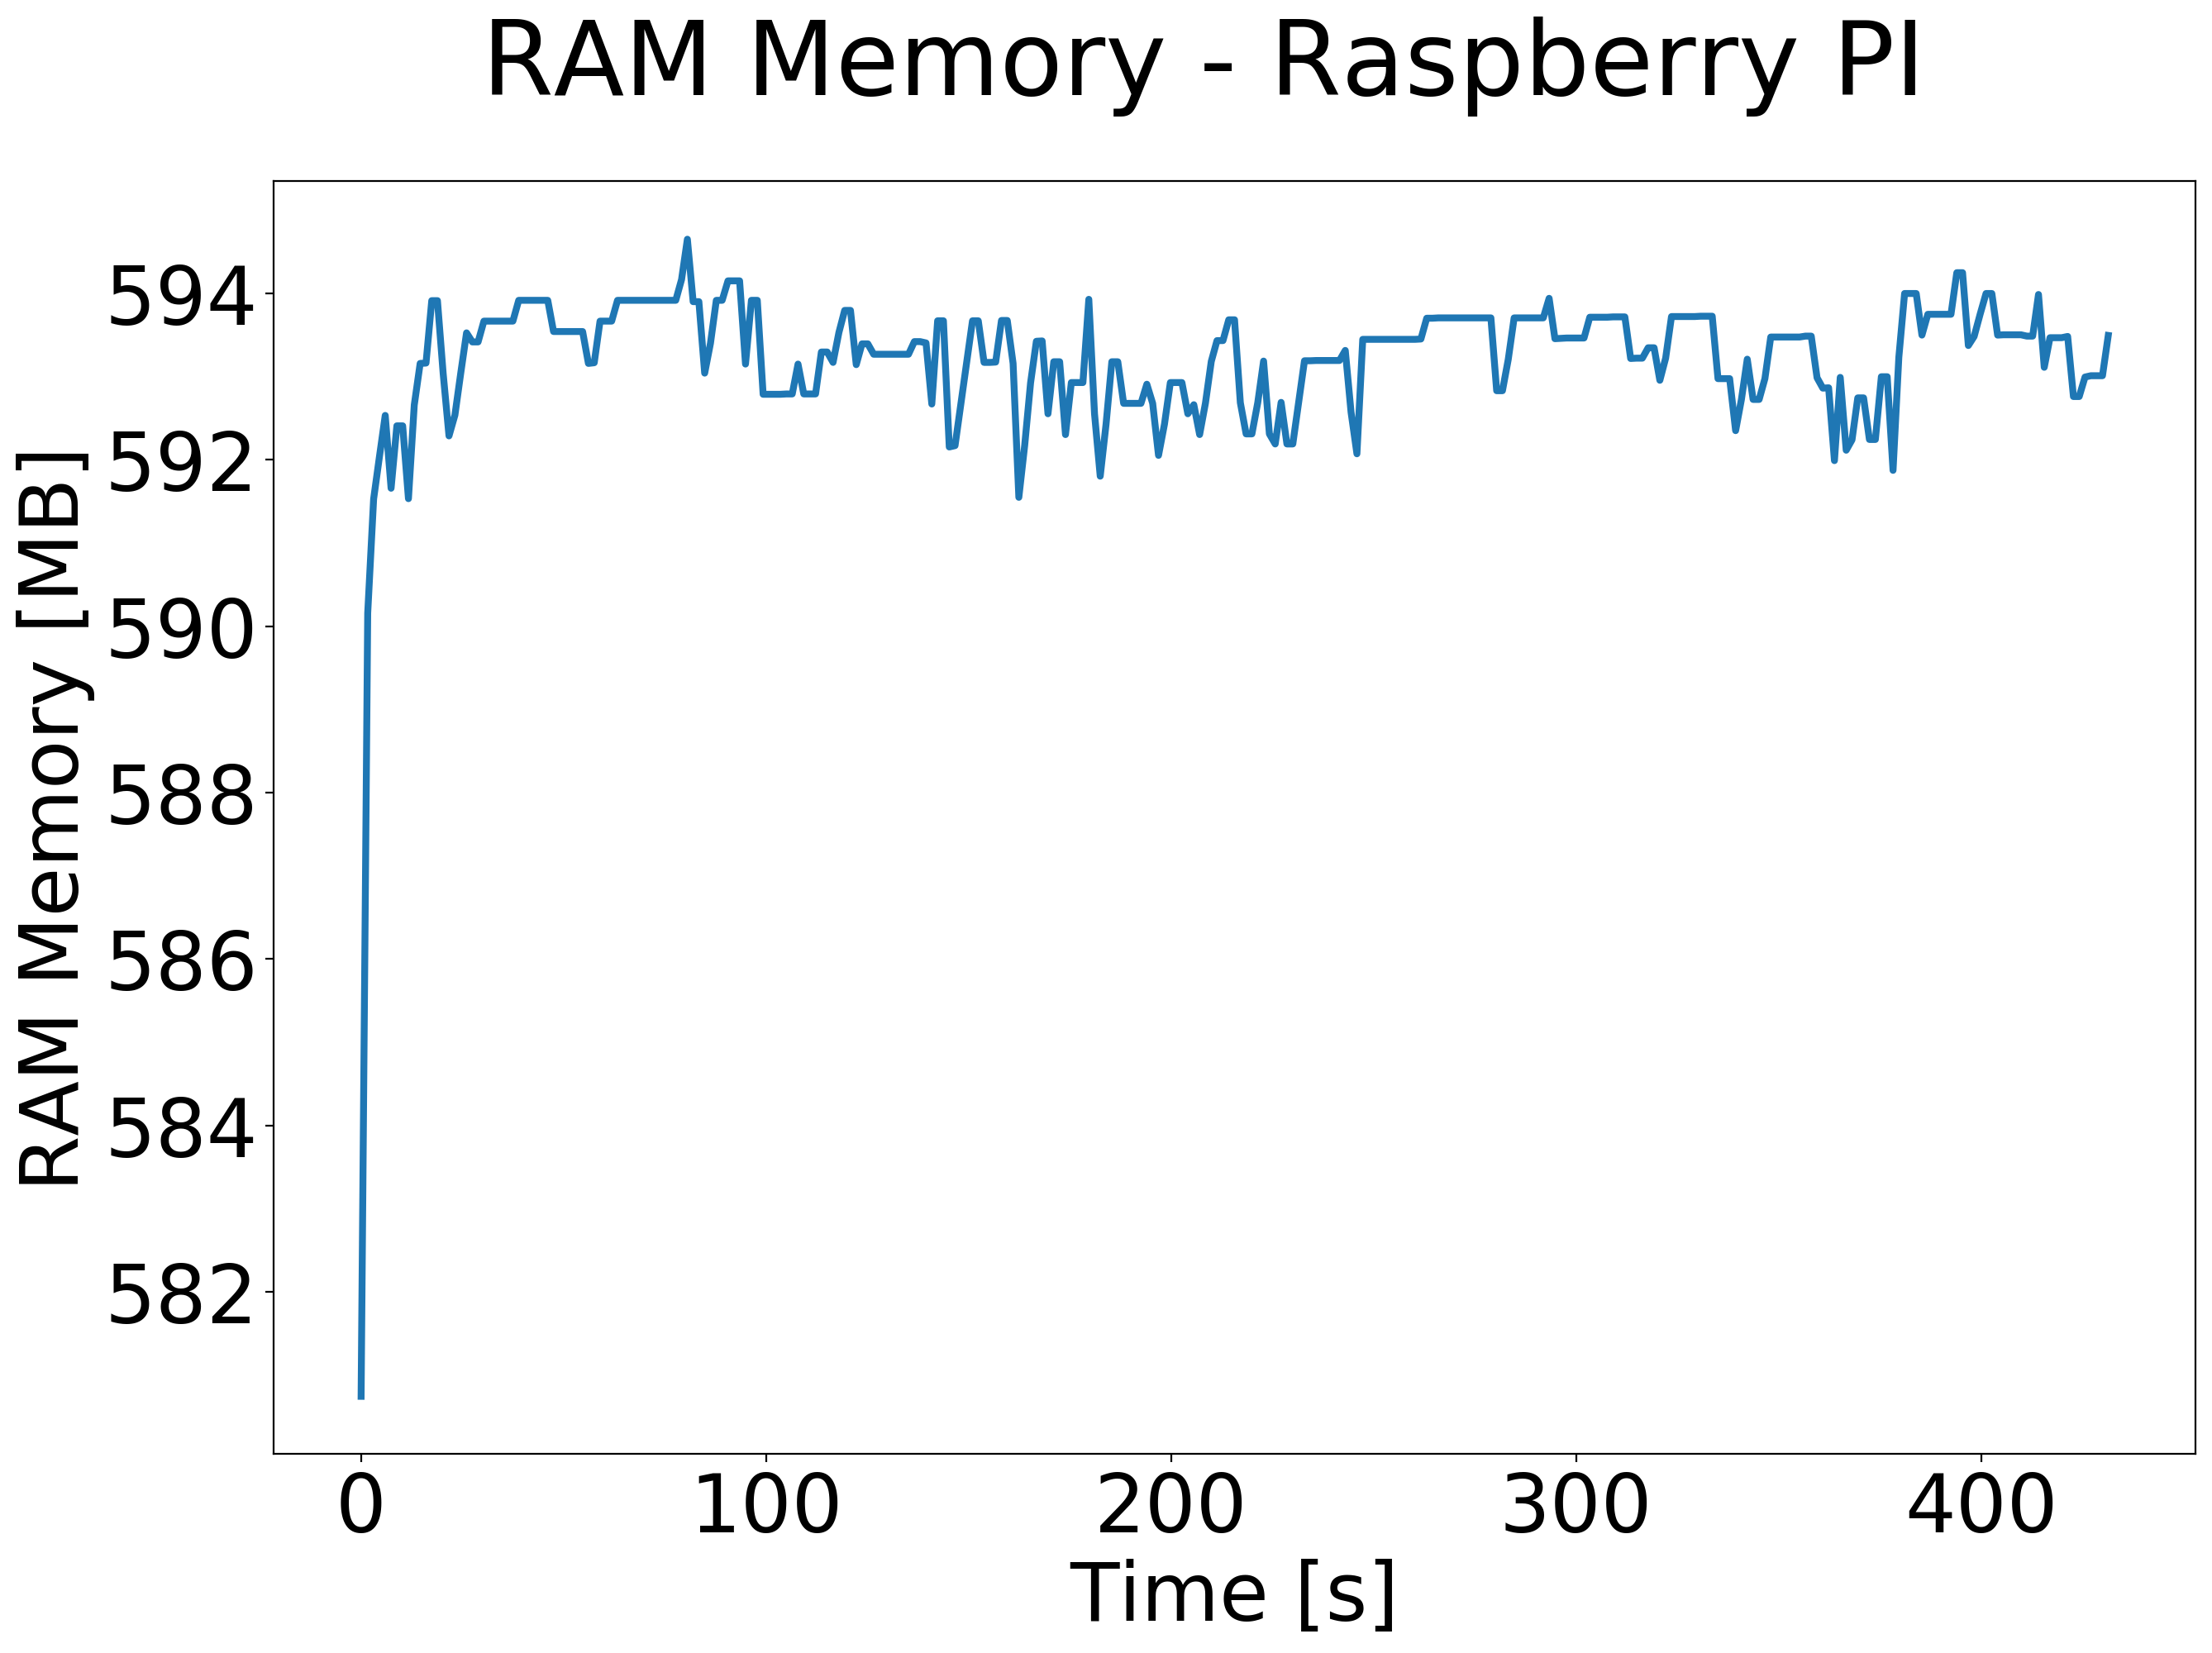
\includegraphics[scale=0.22]{figs/RAM RB.png}}
% \caption{RAM memory in Raspberry PI}
% \label{fig11}
% \end{figure}
% \begin{figure}[htbp]
% \centerline{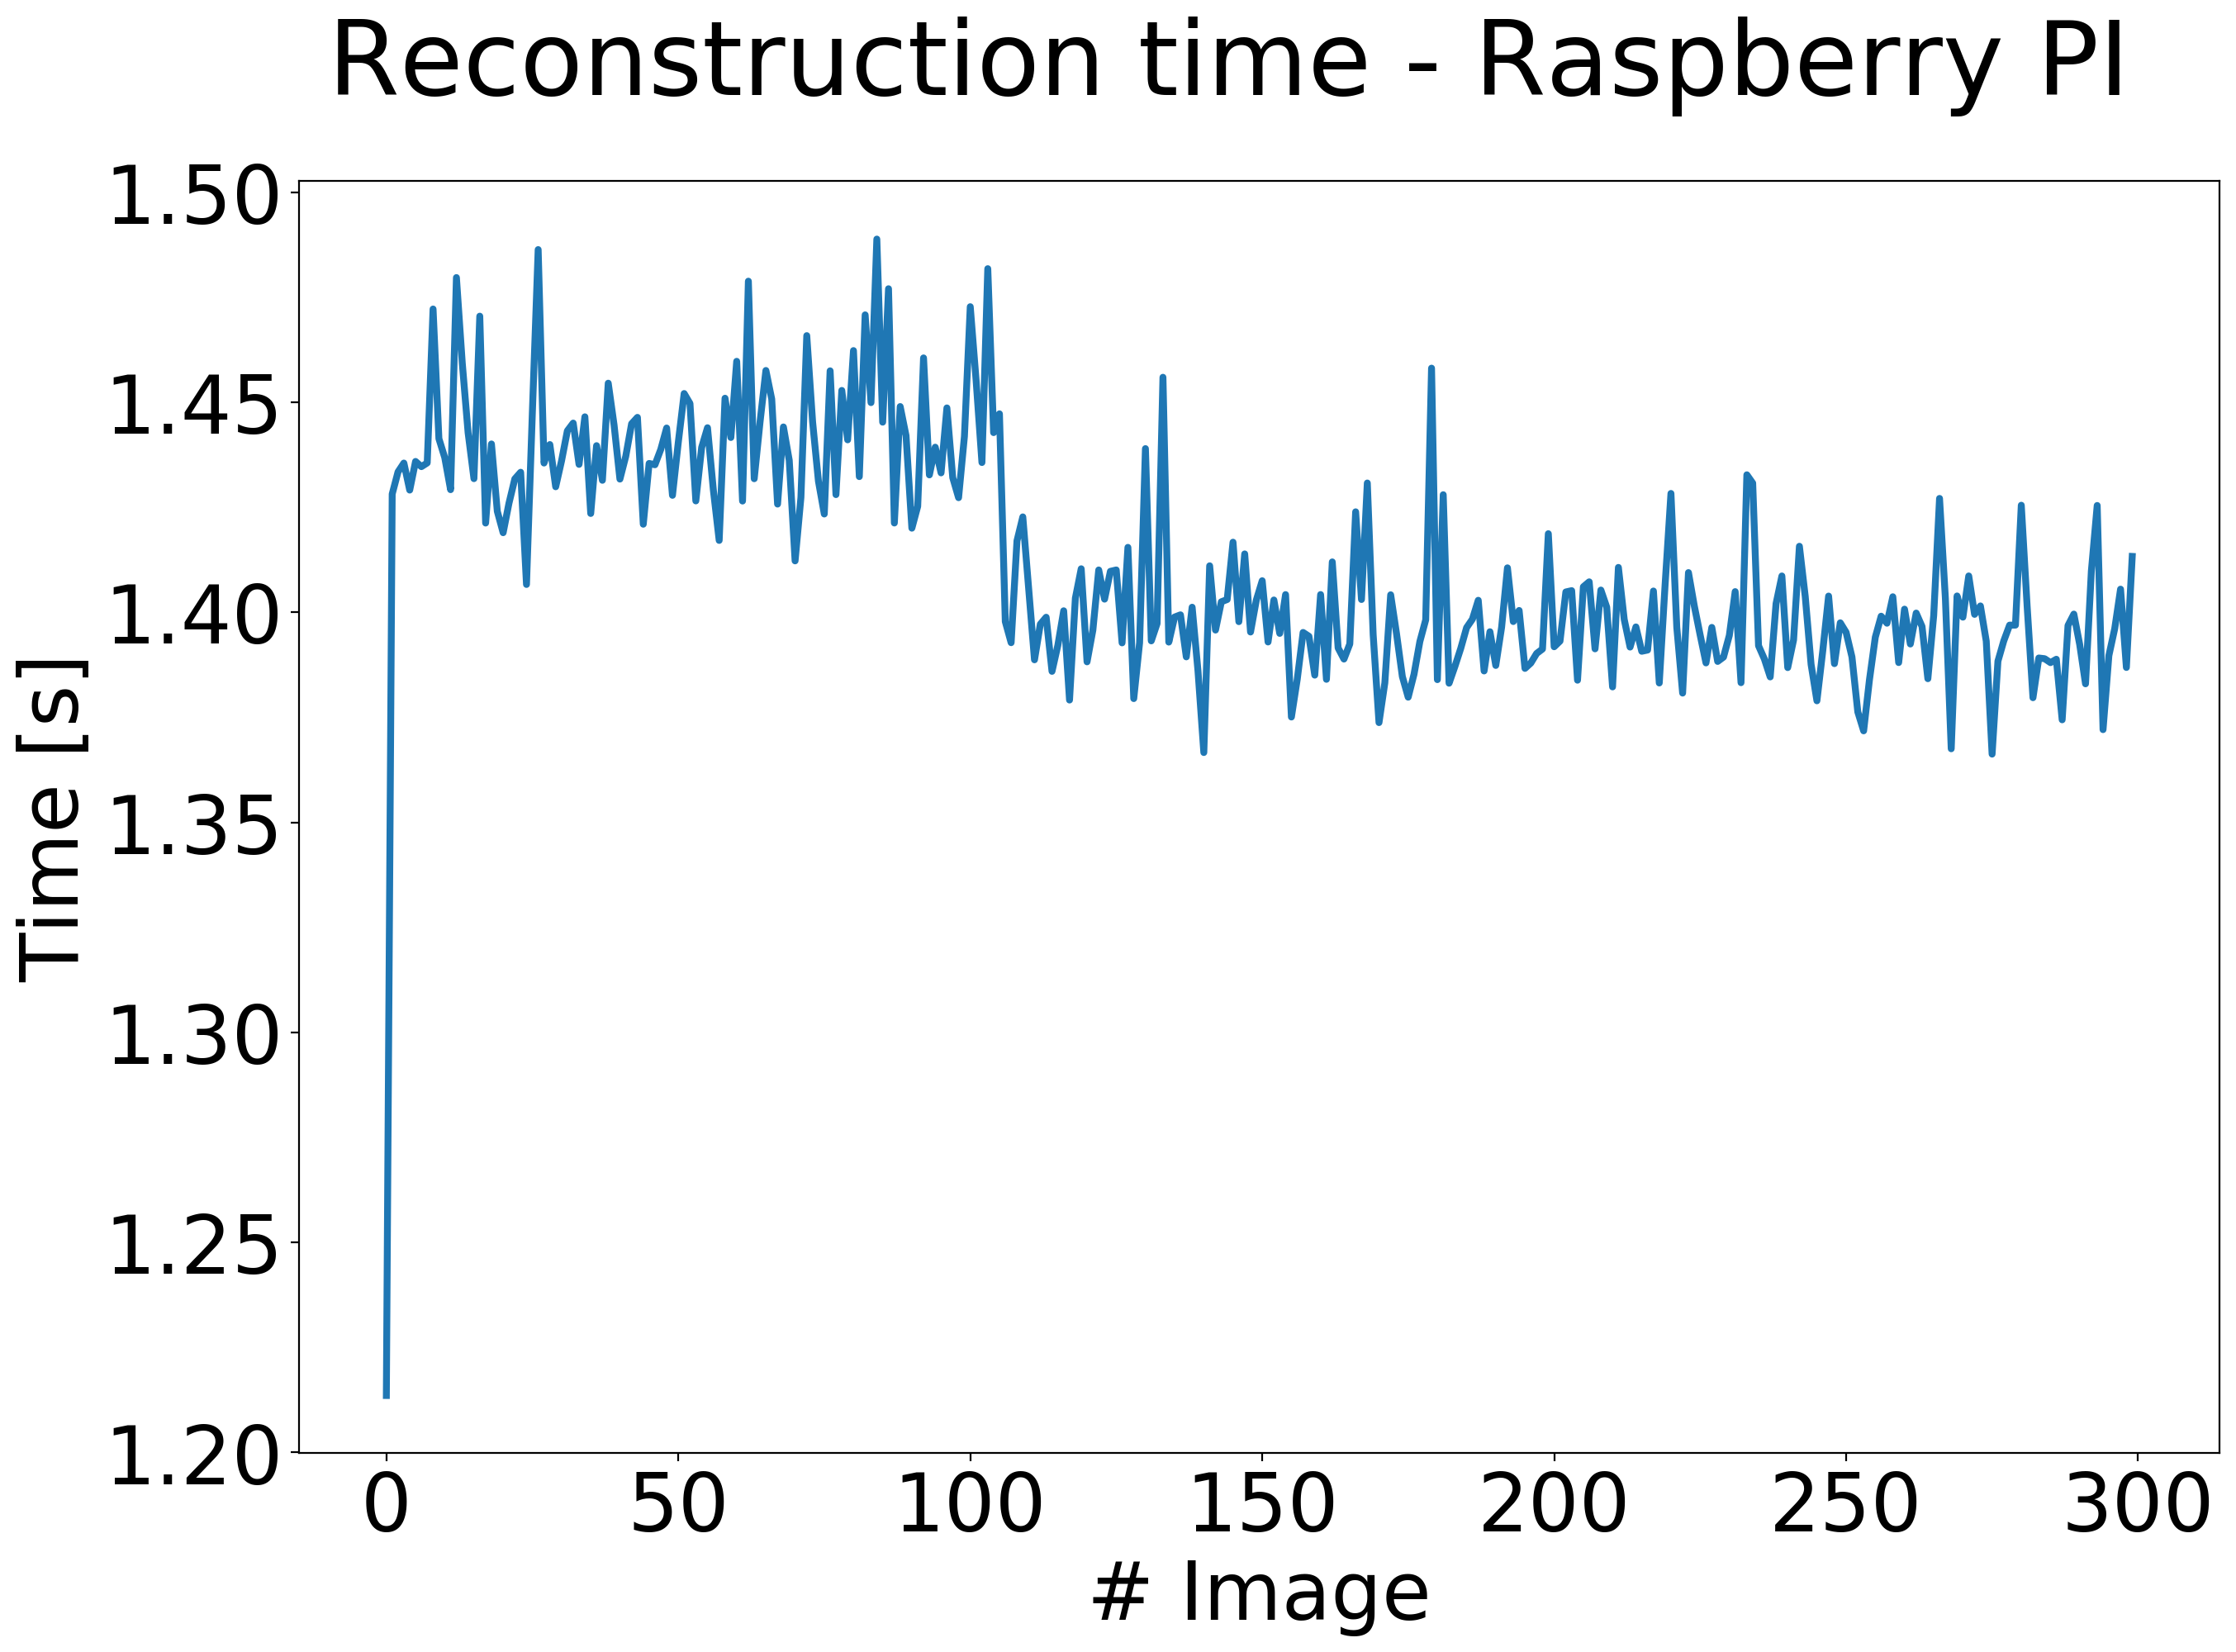
\includegraphics[scale=0.22]{figs/Time RB.png}}
% \caption{Average time in Raspberry PI}
% \label{fig11}
% \end{figure}
% The second engine corresponds to a desktop computer which simulates a server running a fingerprint reconstruction API. RAM memory result is similar to obtained in Raspberry PI experiment since the calculated value is equal to 612 MB. In this case, average reconstruction time per fingerprint was 0.2 seconds.
% \begin{figure}[!ht]
% \centerline{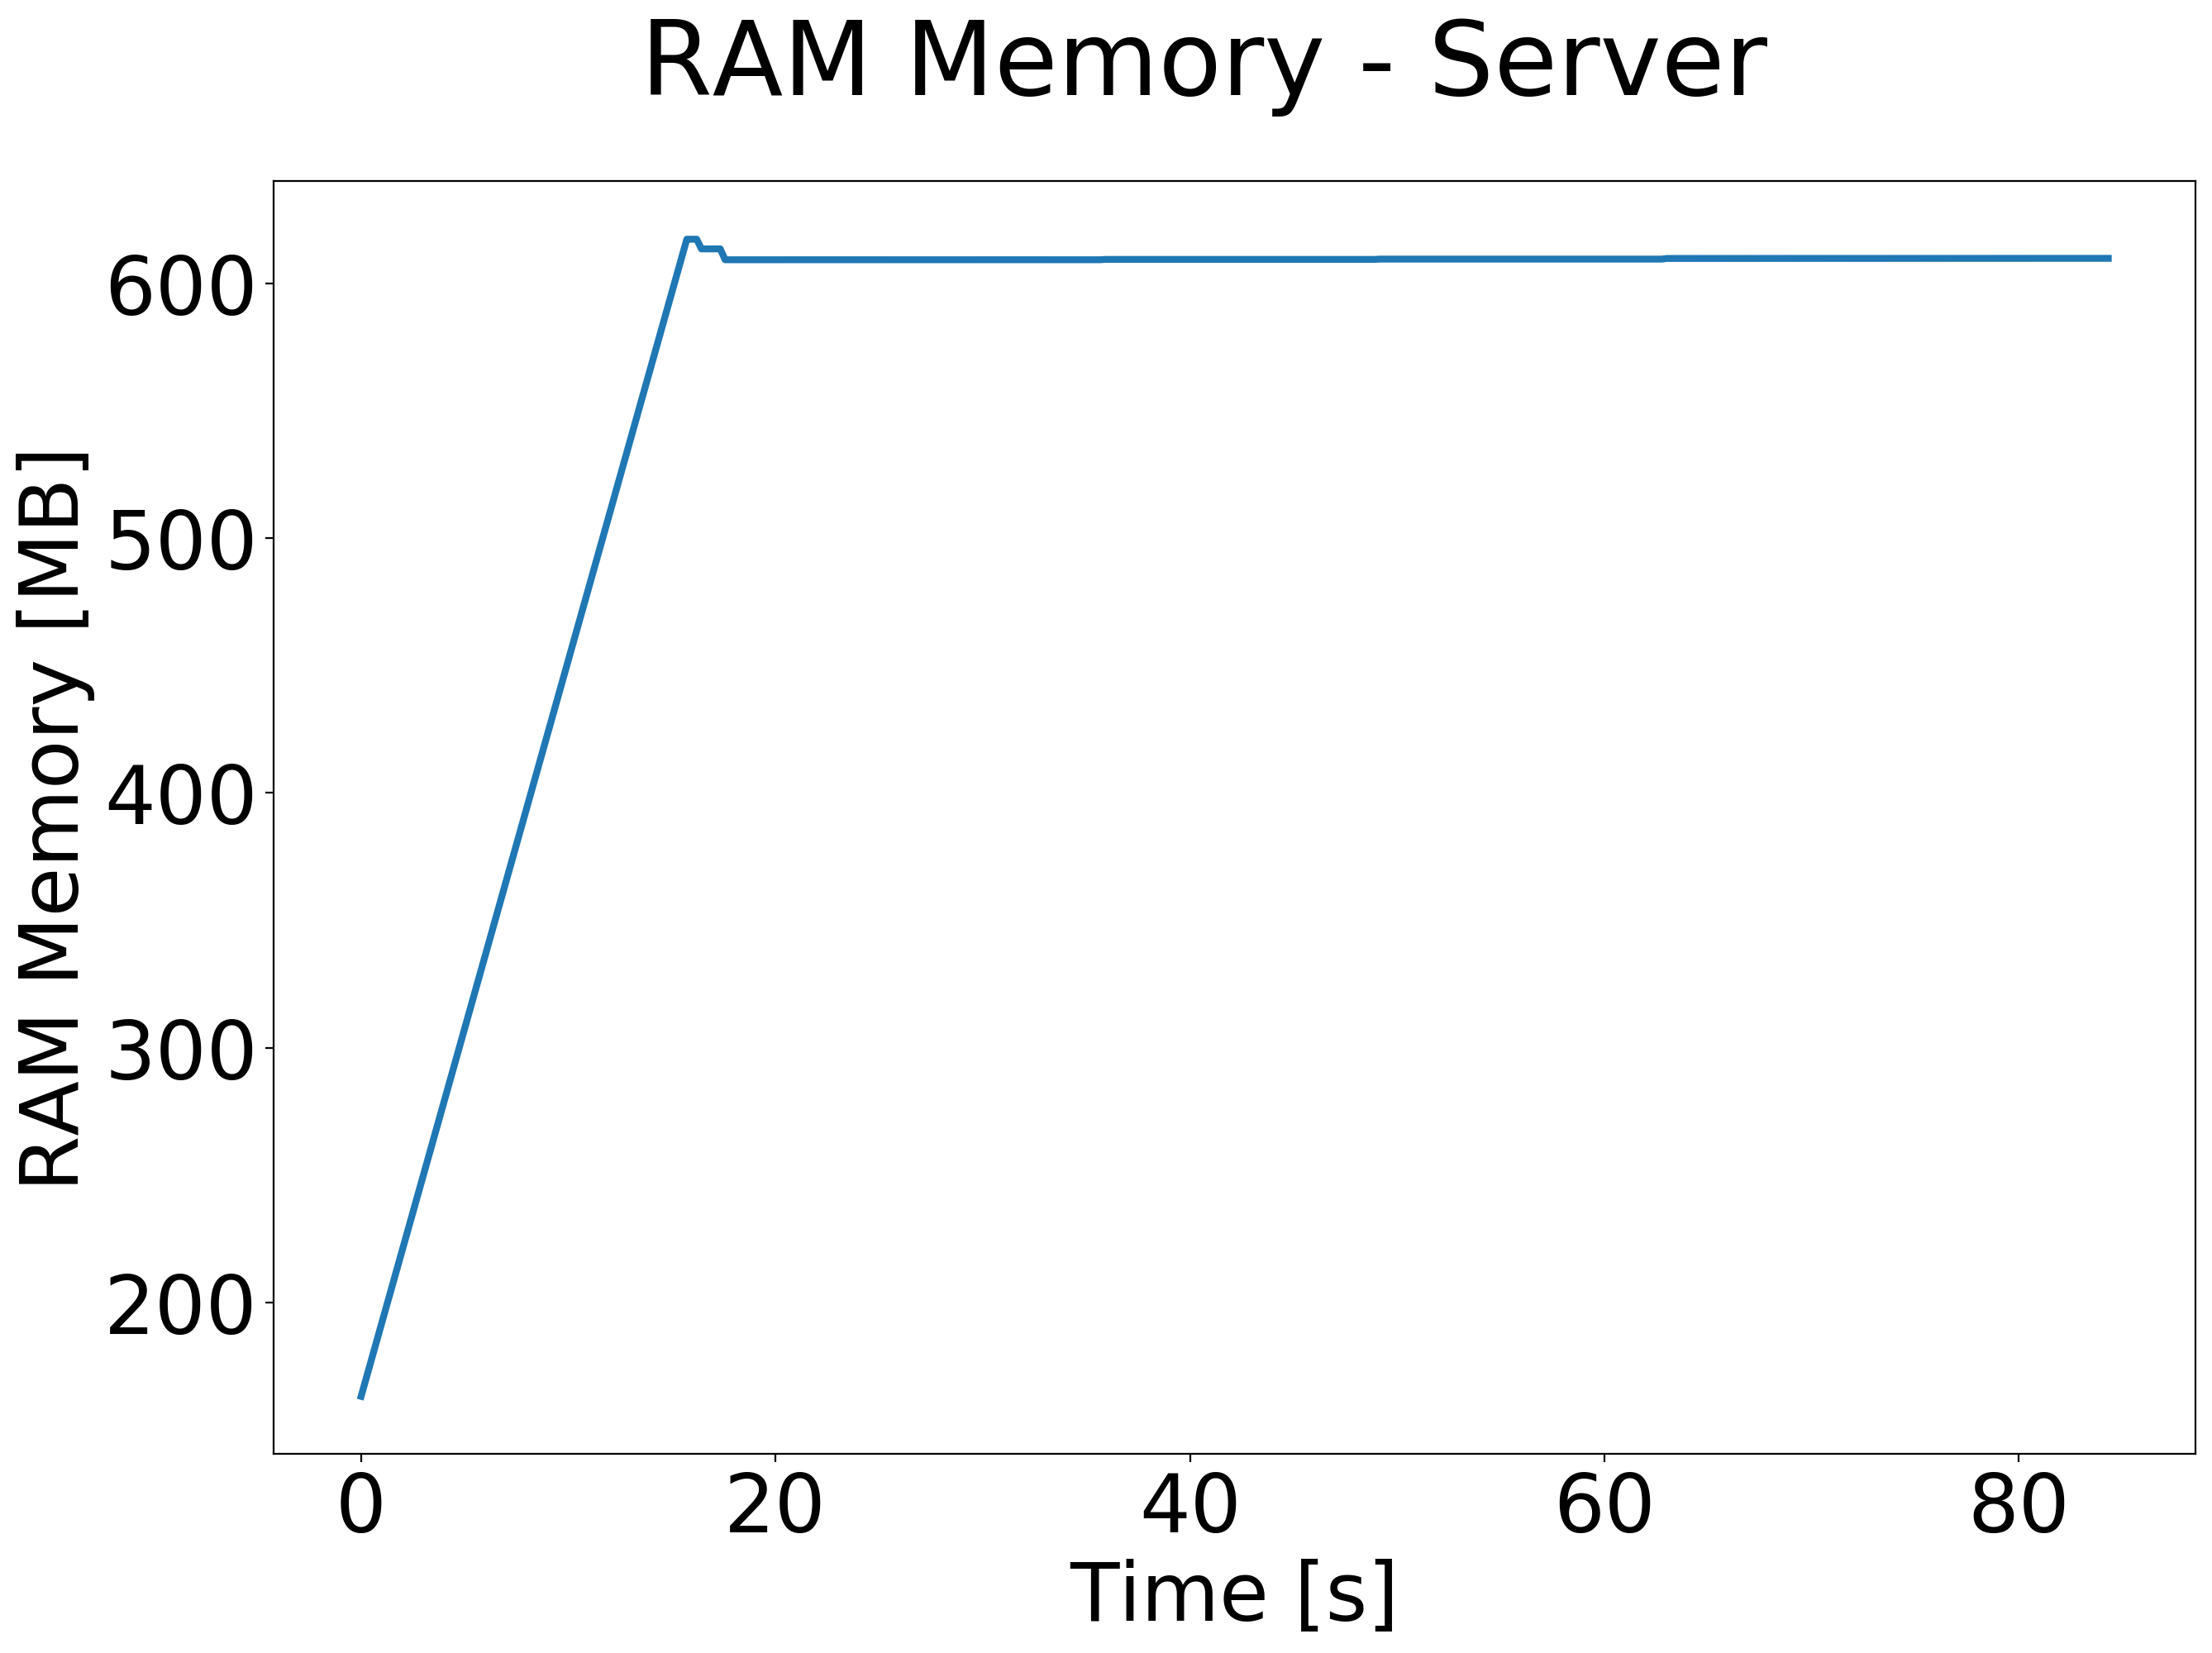
\includegraphics[scale=0.22]{figs/RAM Server.png}}
% \caption{RAM memory in server}
% \label{fig11}
% \end{figure}
% \begin{figure}[!ht]
% \centerline{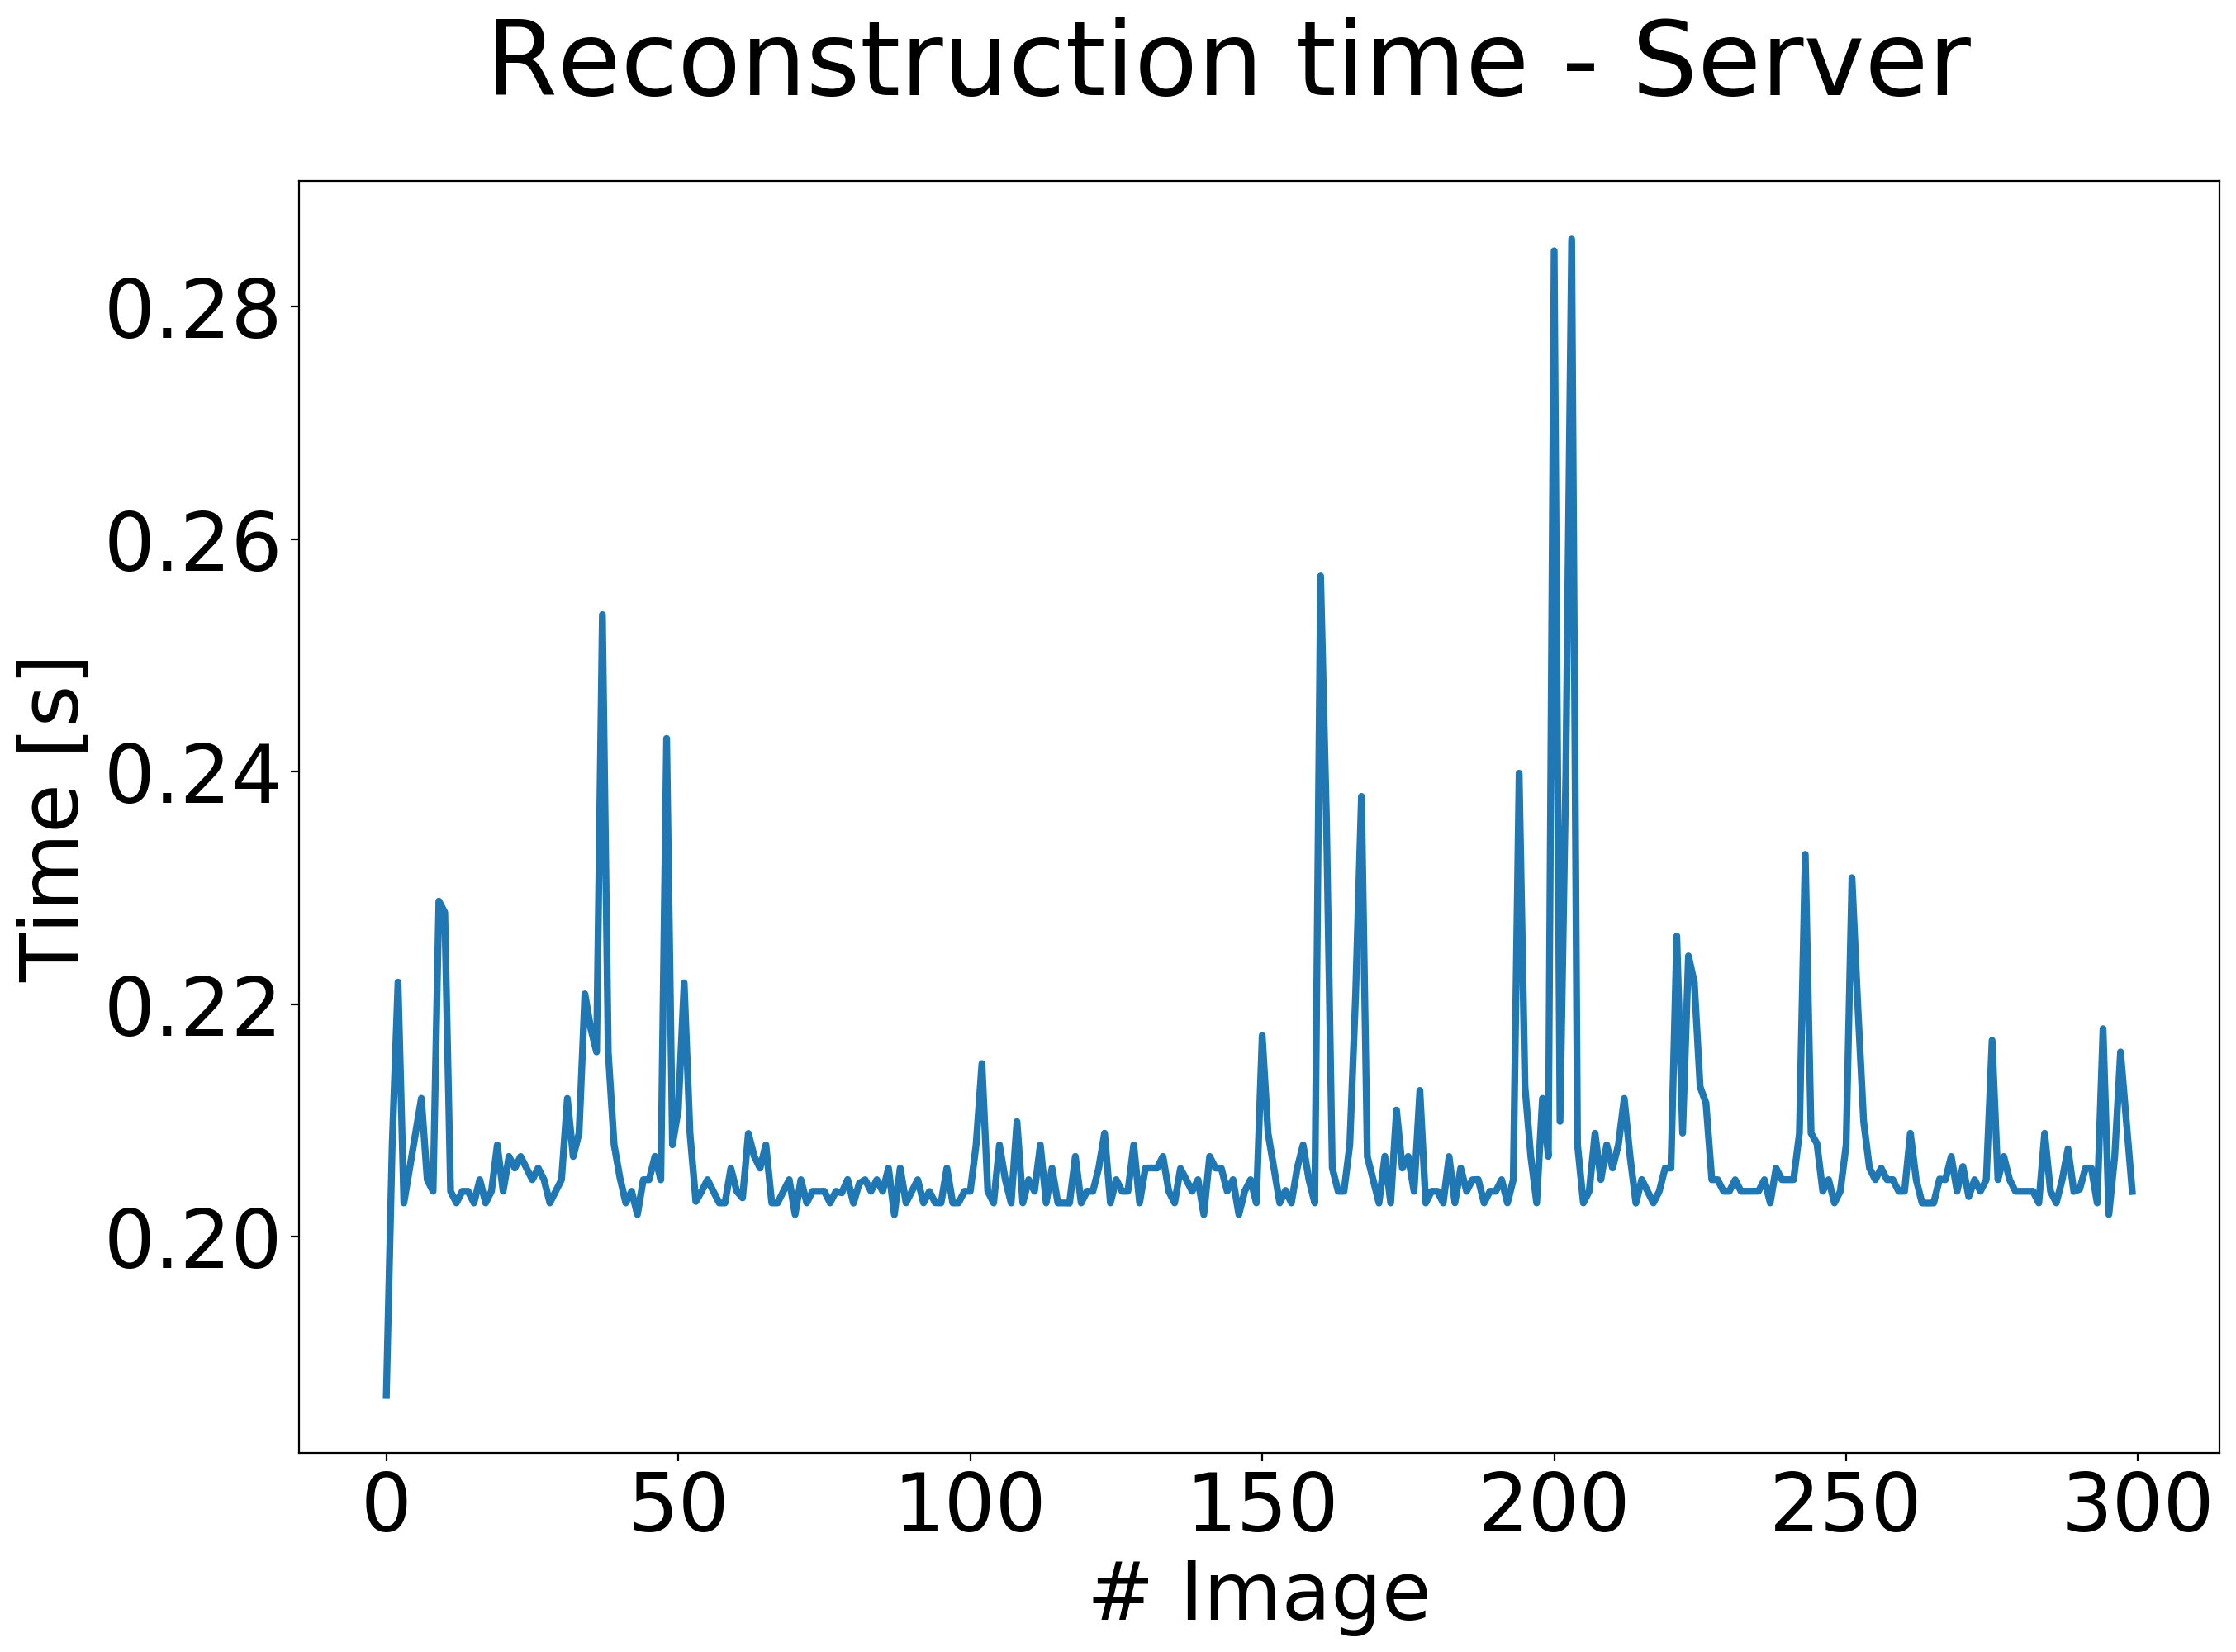
\includegraphics[scale=0.22]{figs/Time Server.png}}
% \caption{Average time in server}
% \label{fig11}
% \end{figure}

%%%%%%%%%%%%%%%%%%%%%%%%%%%%%%%%%%%%%%%%%%%%%
\section{Conclusion}
\label{sec:CON}
\label{sec:FW}
We implemented a \textcolor{green}{generative convolutional neural network that was able to reconstruct deteriorated fingerprints successfully. The model was trained using the adversarial paradigm in which a generator and a discriminator competes to make the model learn the enhancement transformation.} \textcolor{red}{...Resumir aqui lo que se hizo, en tiempo pasado.}. We conducted different tests to evaluate the performance of the proposed model such as ROC and CMC curves, showing an improvement of the quality of the image and matching accuracy after the enhancement process. We also conducted a computational load test to show that the model can be implemented on engines for real-time applications. 


A future research directions, more complex deterioration algorithms can be studied to simulate real world scenarios. Even though it is a challenging task, a dataset containing real corrupted fingerprints and their corresponding ground truth images can be collected. This could be useful to improve generalization and performance of reconstruction models. Also, the proposed model in this paper can be extended to include prior information such as minutae templates and the use of Bayesian inference concepts to define the cost functions, which as proven to be useful in some applications that involve adversarial models.

\printcredits

%% Loading bibliography style file
%\bibliographystyle{model1-num-names}
\bibliographystyle{cas-model2-names}

% Loading bibliography database
\bibliography{cas-refs}

%\vskip3pt

% \bio{figs/foto_cristian.png}
% \textbf{Cristian Yesid Andrade Hernández} courses ninth semester of Electronic Engineering at Universidad de los Andes. Interested in technology applications that involves machine learning, pattern recognition, robotics, control and artificial intelligence. Algorithms and programming skills cover Java, C\#, Python, JavaScript, C++, Visual Basic and Matlab. Two years of experience teaching programming as tutor in a engineering course at university. Internship at Colpatria Group Company: Olimpia IT working on automatic testing of the software.
% \endbio

\onecolumn
\appendix
\section{My Appendix}

\begin{table}[htbp]
\caption{Architecture details of generator}
\begin{tabular}{|c|c|c|c|c|c|c|c|c|}
\hline
{\color[HTML]{000000} \textbf{Layer}} &
  {\color[HTML]{000000} \textbf{Strides}} &
  {\color[HTML]{000000} \textbf{Padding}} &
  {\color[HTML]{000000} \textbf{Filters}} &
  {\color[HTML]{000000} \textbf{Input size}} &
  {\color[HTML]{000000} \textbf{Output size}} &
  {\color[HTML]{000000} \textbf{Batchnorm}} &
  {\color[HTML]{000000} \textbf{Activation}} &
  {\color[HTML]{000000} \textbf{Dropout}} \\ \hline
{\color[HTML]{000000} Conv1} &
  {\color[HTML]{000000} (4,4)} &
  {\color[HTML]{000000} same} &
  {\color[HTML]{000000} 64} &
  {\color[HTML]{000000} (256,256,1)} &
  {\color[HTML]{000000} (128,128,64)} &
  {\color[HTML]{000000} No} &
  {\color[HTML]{000000} LeakyRelu} &
  {\color[HTML]{000000} No} \\ \hline
{\color[HTML]{000000} Conv2} &
  {\color[HTML]{000000} (4,4)} &
  {\color[HTML]{000000} same} &
  {\color[HTML]{000000} 128} &
  {\color[HTML]{000000} (128,128,64)} &
  {\color[HTML]{000000} (64,64,128)} &
  {\color[HTML]{000000} Yes} &
  {\color[HTML]{000000} LeakyRelu} &
  {\color[HTML]{000000} No} \\ \hline
{\color[HTML]{000000} Conv3} &
  {\color[HTML]{000000} (4,4)} &
  {\color[HTML]{000000} same} &
  {\color[HTML]{000000} 256} &
  {\color[HTML]{000000} (64,64,128)} &
  {\color[HTML]{000000} (32,32,256)} &
  {\color[HTML]{000000} Yes} &
  {\color[HTML]{000000} LeakyRelu} &
  {\color[HTML]{000000} No} \\ \hline
{\color[HTML]{000000} Conv4} &
  {\color[HTML]{000000} (4,4)} &
  {\color[HTML]{000000} same} &
  {\color[HTML]{000000} 512} &
  {\color[HTML]{000000} (32,32,256)} &
  {\color[HTML]{000000} (16,16,512)} &
  {\color[HTML]{000000} Yes} &
  {\color[HTML]{000000} LeakyRelu} &
  {\color[HTML]{000000} No} \\ \hline
{\color[HTML]{000000} Conv5} &
  {\color[HTML]{000000} (4,4)} &
  {\color[HTML]{000000} same} &
  {\color[HTML]{000000} 512} &
  {\color[HTML]{000000} (16,16,512)} &
  {\color[HTML]{000000} (8,8,512)} &
  {\color[HTML]{000000} Yes} &
  {\color[HTML]{000000} LeakyRelu} &
  {\color[HTML]{000000} No} \\ \hline
{\color[HTML]{000000} Conv6} &
  {\color[HTML]{000000} (4,4)} &
  {\color[HTML]{000000} same} &
  {\color[HTML]{000000} 512} &
  {\color[HTML]{000000} (8,8,512)} &
  {\color[HTML]{000000} (4,4,512)} &
  {\color[HTML]{000000} Yes} &
  {\color[HTML]{000000} LeakyRelu} &
  {\color[HTML]{000000} No} \\ \hline
{\color[HTML]{000000} Conv7} &
  {\color[HTML]{000000} (4,4)} &
  {\color[HTML]{000000} same} &
  {\color[HTML]{000000} 512} &
  {\color[HTML]{000000} (4,4,512)} &
  {\color[HTML]{000000} (2,2,512)} &
  {\color[HTML]{000000} Yes} &
  {\color[HTML]{000000} LeakyRelu} &
  {\color[HTML]{000000} No} \\ \hline
{\color[HTML]{000000} Conv8} &
  {\color[HTML]{000000} (4,4)} &
  {\color[HTML]{000000} same} &
  {\color[HTML]{000000} 512} &
  {\color[HTML]{000000} (2,2,512)} &
  {\color[HTML]{000000} (1,1,512)} &
  {\color[HTML]{000000} Yes} &
  {\color[HTML]{000000} LeakyRelu} &
  {\color[HTML]{000000} No} \\ \hline
{\color[HTML]{000000} TransConv1} &
  {\color[HTML]{000000} (4,4)} &
  {\color[HTML]{000000} same} &
  {\color[HTML]{000000} 512} &
  {\color[HTML]{000000} (1,1,512)} &
  {\color[HTML]{000000} (2,2,512)} &
  {\color[HTML]{000000} Yes} &
  {\color[HTML]{000000} Relu} &
  {\color[HTML]{000000} Yes} \\ \hline
{\color[HTML]{000000} TransConv2} &
  {\color[HTML]{000000} (4,4)} &
  {\color[HTML]{000000} same} &
  {\color[HTML]{000000} 512} &
  {\color[HTML]{000000} (2,2,512)} &
  {\color[HTML]{000000} (4,4,512)} &
  {\color[HTML]{000000} Yes} &
  {\color[HTML]{000000} Relu} &
  {\color[HTML]{000000} Yes} \\ \hline
{\color[HTML]{000000} TransConv3} &
  {\color[HTML]{000000} (4,4)} &
  {\color[HTML]{000000} same} &
  {\color[HTML]{000000} 512} &
  {\color[HTML]{000000} (4,4,512)} &
  {\color[HTML]{000000} (8,8,512)} &
  {\color[HTML]{000000} Yes} &
  {\color[HTML]{000000} Relu} &
  {\color[HTML]{000000} Yes} \\ \hline
{\color[HTML]{000000} TransConv4} &
  {\color[HTML]{000000} (4,4)} &
  {\color[HTML]{000000} same} &
  {\color[HTML]{000000} 512} &
  {\color[HTML]{000000} (8,8,512)} &
  {\color[HTML]{000000} (16,16,512)} &
  {\color[HTML]{000000} Yes} &
  {\color[HTML]{000000} Relu} &
  {\color[HTML]{000000} No} \\ \hline
{\color[HTML]{000000} TransConv5} &
  {\color[HTML]{000000} (4,4)} &
  {\color[HTML]{000000} same} &
  {\color[HTML]{000000} 256} &
  {\color[HTML]{000000} (16,16,512)} &
  {\color[HTML]{000000} (32,32,256)} &
  {\color[HTML]{000000} Yes} &
  {\color[HTML]{000000} Relu} &
  {\color[HTML]{000000} No} \\ \hline
{\color[HTML]{000000} TransConv6} &
  {\color[HTML]{000000} (4,4)} &
  {\color[HTML]{000000} same} &
  {\color[HTML]{000000} 128} &
  {\color[HTML]{000000} (32,32,256)} &
  {\color[HTML]{000000} (64,64,128)} &
  {\color[HTML]{000000} Yes} &
  {\color[HTML]{000000} Relu} &
  {\color[HTML]{000000} No} \\ \hline
{\color[HTML]{000000} TransConv7} &
  {\color[HTML]{000000} (4,4)} &
  {\color[HTML]{000000} same} &
  {\color[HTML]{000000} 64} &
  {\color[HTML]{000000} (64,64,128)} &
  {\color[HTML]{000000} (128,128,64)} &
  {\color[HTML]{000000} Yes} &
  {\color[HTML]{000000} Relu} &
  {\color[HTML]{000000} No} \\ \hline
{\color[HTML]{000000} TransConv8} &
  {\color[HTML]{000000} (4,4)} &
  {\color[HTML]{000000} same} &
  {\color[HTML]{000000} 1} &
  {\color[HTML]{000000} (128,128,64)} &
  {\color[HTML]{000000} (256,256,1)} &
  {\color[HTML]{000000} Yes} &
  {\color[HTML]{000000} Tanh} &
  {\color[HTML]{000000} No} \\ \hline
\end{tabular}
\label{tab1}
\end{table}

\begin{table}[htbp]
\caption{Architecture details of discriminator}
\begin{tabular}{|c|c|c|c|c|c|c|c|c|}
\hline
{\color[HTML]{000000} \textbf{Layer}} &
  {\color[HTML]{000000} \textbf{Strides}} &
  {\color[HTML]{000000} \textbf{Padding}} &
  {\color[HTML]{000000} \textbf{Filters}} &
  {\color[HTML]{000000} \textbf{Input size}} &
  {\color[HTML]{000000} \textbf{Output size}} &
  {\color[HTML]{000000} \textbf{Batchnorm}} &
  {\color[HTML]{000000} \textbf{Activation}} &
  {\color[HTML]{000000} \textbf{Dropout}} \\ \hline
{\color[HTML]{000000} Conv1} &
  {\color[HTML]{000000} (4,4)} &
  {\color[HTML]{000000} same} &
  {\color[HTML]{000000} 64} &
  {\color[HTML]{000000} (256,256,1)} &
  {\color[HTML]{000000} (128,128,64)} &
  {\color[HTML]{000000} Yes} &
  {\color[HTML]{000000} LeakyRelu} &
  {\color[HTML]{000000} No} \\ \hline
{\color[HTML]{000000} Conv2} &
  {\color[HTML]{000000} (4,4)} &
  {\color[HTML]{000000} same} &
  {\color[HTML]{000000} 128} &
  {\color[HTML]{000000} (128,128,64)} &
  {\color[HTML]{000000} (64,64,128)} &
  {\color[HTML]{000000} Yes} &
  {\color[HTML]{000000} LeakyRelu} &
  {\color[HTML]{000000} No} \\ \hline
{\color[HTML]{000000} Conv3} &
  {\color[HTML]{000000} (4,4)} &
  {\color[HTML]{000000} same} &
  {\color[HTML]{000000} 256} &
  {\color[HTML]{000000} (64,64,128)} &
  {\color[HTML]{000000} (32,32,256)} &
  {\color[HTML]{000000} Yes} &
  {\color[HTML]{000000} LeakyRelu} &
  {\color[HTML]{000000} No} \\ \hline
{\color[HTML]{000000} Con4} &
  {\color[HTML]{000000} (1,1)} &
  {\color[HTML]{000000} same} &
  {\color[HTML]{000000} 512} &
  {\color[HTML]{000000} (32,32,256)} &
  {\color[HTML]{000000} (32,32,512)} &
  {\color[HTML]{000000} Yes} &
  {\color[HTML]{000000} LeakyRelu} &
  {\color[HTML]{000000} No} \\ \hline
{\color[HTML]{000000} Conv5} &
  {\color[HTML]{000000} (1,1)} &
  {\color[HTML]{000000} same} &
  {\color[HTML]{000000} 1} &
  {\color[HTML]{000000} (32,32,512)} &
  {\color[HTML]{000000} (29,29,1)} &
  {\color[HTML]{000000} No} &
  {\color[HTML]{000000} None} &
  {\color[HTML]{000000} No} \\ \hline
\end{tabular}
\label{tab2}
\end{table}

\begin{figure}[htbp]
\centerline{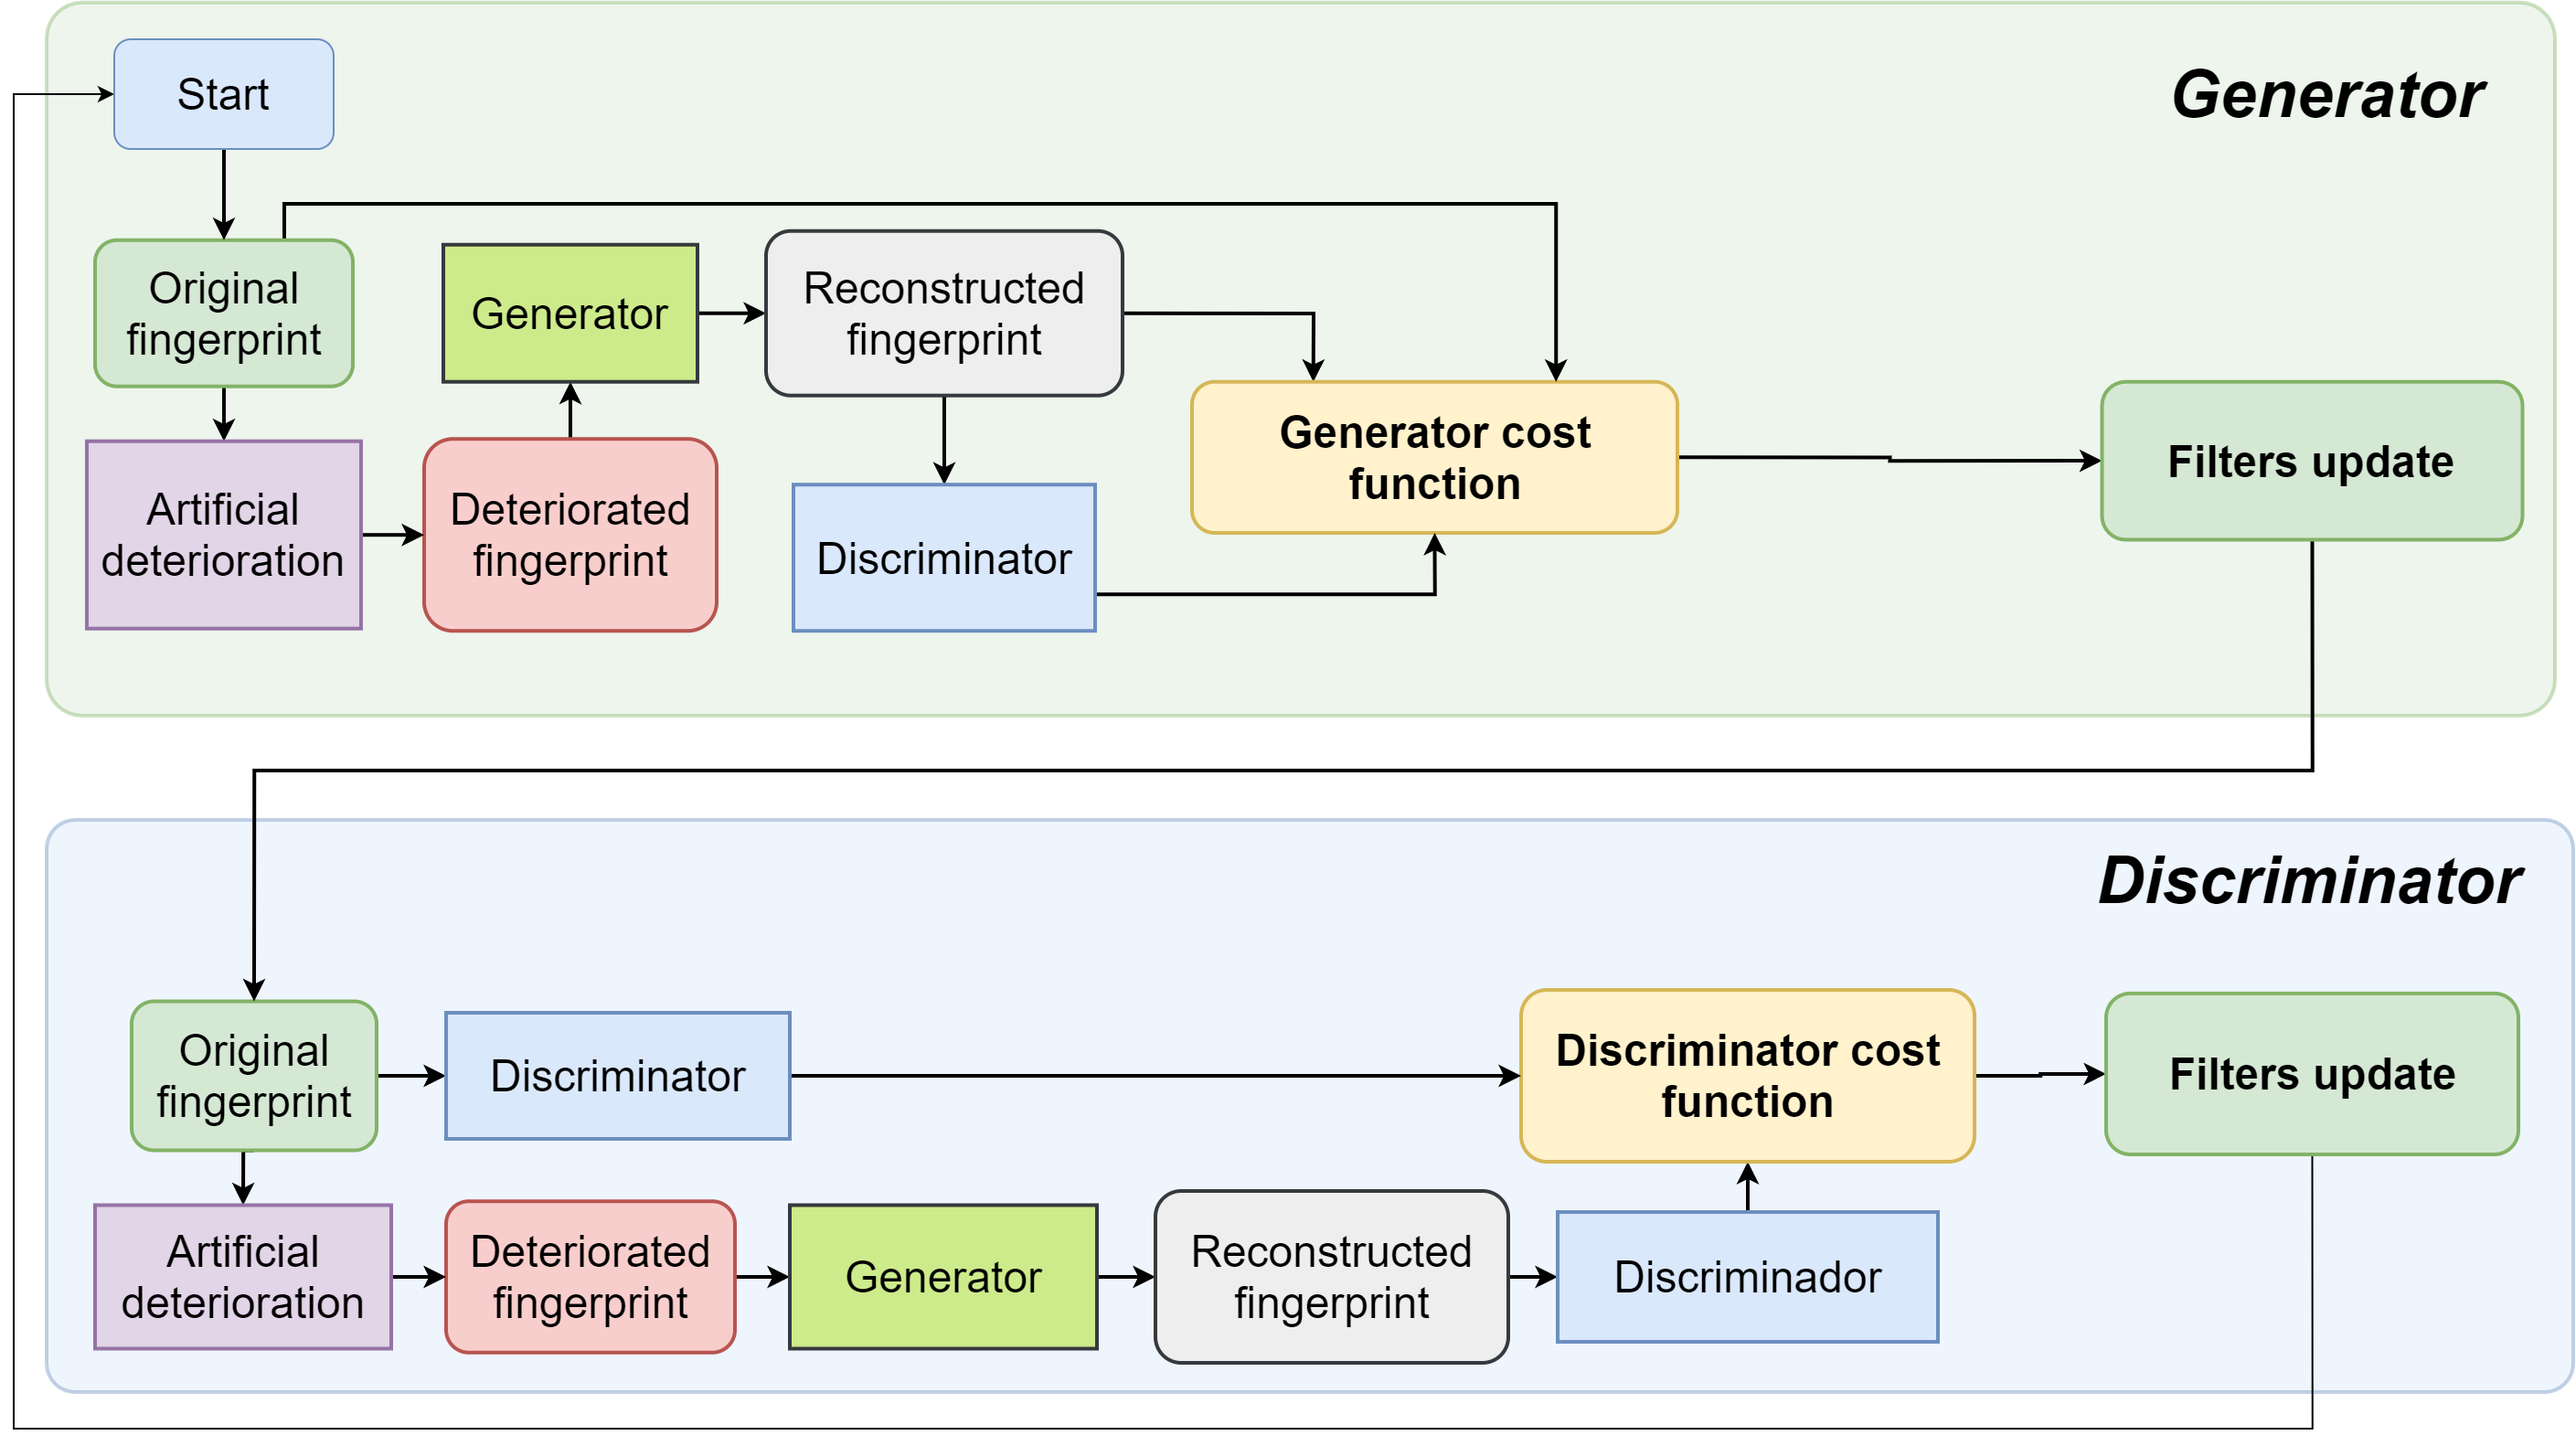
\includegraphics[scale=0.4]{figs/training_fd_en_h.png}}
\caption{Training flow \textcolor{red}{y esta grafica donde iria??} \textcolor{green}{es la misma de arriba. Sucede que no sabía cuál de las dos poner. Supongo que se puede quitar}}
\end{figure}

\end{document}